\documentclass[a4paper,style=print,bibliography=totoc,nexus,lnum,extramargin]{tubsbook}

%\usepackage[T1]{fontenc}
\usepackage[utf8]{inputenc}

\usepackage{float}
%\usepackage{pgfplots}
\usepackage{microtype}
\usepackage{xcolor}
    \definecolor{medium-blue}{rgb}{0,0,0.5}
\usepackage{algorithm}
\usepackage{algpseudocode}
    \renewcommand{\algorithmicrequire}{\textbf{Input:}}
    \renewcommand{\algorithmicensure}{\textbf{Output:}}
\usepackage{hyperref}
\usepackage{amsmath}
\usepackage{amsthm}
\usepackage{mathtools}
    \mathtoolsset{centercolon}
\usepackage[nameinlink]{cleveref}
    \newtheorem{theorem}{Theorem}
    \newtheorem{corollary}{Corollary}
    \theoremstyle{definition}
    \newtheorem{definition}{Definition}
    \newtheorem{lemma}{Lemma}
    \newtheorem{problem}{Problem}
    \newtheorem{conjecture}{Conjecture}
\usepackage{amsfonts}
%\usepackage{todonotes}
\usepackage{subcaption}
\usepackage{tikz}
    \usetikzlibrary{calc}
    \usetikzlibrary{arrows}
    \usetikzlibrary{decorations.pathreplacing}
    %\usetikzlibrary{external}
    %\tikzexternalize[prefix=tikz/]
    \newcommand\fig[3][3]{%
        \begin{figure}%
            %\tikzsetnextfilename{#1}%
            \begin{tikzpicture}[scale=#1]%
                \input{tikz/#2.tex}%
            \end{tikzpicture}%
            \caption{#3}%
            \label{fig:#2}%
        \end{figure}%
    }
    \newcommand\subfig[2][3]{%
        %\tikzsetnextfilename{#1}%
        \begin{tikzpicture}[scale=#1]%
            \input{tikz/#2.tex}%
        \end{tikzpicture}%
    }
\usepackage{graphicx}
    \graphicspath{{images/}}
\usepackage{longtable}
    \renewcommand{\arraystretch}{2}
\usepackage{chngcntr}
    \counterwithout{equation}{chapter}
\usepackage{nicefrac}
\usepackage{csquotes}
\usepackage{scrhack}
\usepackage{array}
\usepackage{xifthen}
\usepackage[backend=biber,style=numeric-comp,maxbibnames=99,url=false]{biblatex}
    \addbibresource{references.bib}

    %% Link complete "Author (Year)", not just "(Year)"
    %\DeclareFieldFormat{citehyperref}{%
    %  \DeclareFieldAlias{bibhyperref}{noformat}% Avoid nested links
    %  \bibhyperref{#1}}

    %\DeclareFieldFormat{textcitehyperref}{%
    %  \DeclareFieldAlias{bibhyperref}{noformat}% Avoid nested links
    %  \bibhyperref{%
    %    #1%
    %    \ifbool{cbx:parens}
    %      {\bibcloseparen\global\boolfalse{cbx:parens}}
    %      {}}}

    %\savebibmacro{cite}
    %\savebibmacro{textcite}

    %\renewbibmacro*{cite}{%
    %  \printtext[citehyperref]{%
    %    \restorebibmacro{cite}%
    %    \usebibmacro{cite}}}

    %\renewbibmacro*{textcite}{%
    %  \ifboolexpr{
    %    ( not test {\iffieldundef{prenote}} and
    %      test {\ifnumequal{\value{citecount}}{1}} )
    %    or
    %    ( not test {\iffieldundef{postnote}} and
    %      test {\ifnumequal{\value{citecount}}{\value{citetotal}}} )
    %  }
    %    {\DeclareFieldAlias{textcitehyperref}{noformat}}
    %    {}%
    %  \printtext[textcitehyperref]{%
    %    \restorebibmacro{textcite}%
    %    \usebibmacro{textcite}}}

\widowpenalty10000
\clubpenalty10000

\newcommand{\C}{\mathbb{C}}
\newcommand{\R}{\mathbb{R}}
\newcommand{\myS}{\mathbb{S}}
\newcommand{\s}{\sqrt{2}}
\newcommand{\wlofg}{without loss of generality}
\DeclareMathOperator{\mysum}{sum}
\DeclareMathOperator*{\argmin}{arg\,min}

\newcommand{\entry}[7]{
\begin{tikzpicture}[scale=#1,baseline={([yshift={-\ht\strutbox}]current bounding box.north)}]\input{tikz/#2.tex}\end{tikzpicture}
& \textbf{#3} (#4) \vfill\vspace{10pt}
\ifthenelse{\isempty{#5}}{}{\textit{Condition:} #5 \vfill\vspace{5pt}}
\textit{Density:} #6 \vfill\vspace{5pt}
\textit{Approximation factor:} #7\\
}

\makeatletter
    % center the contents of floatstuff automatically
    \g@addto@macro\@floatboxreset\centering

    % set default placement for floatstuff
    \def\fps@figure{H}
    \def\fps@table{H}
    \def\fps@algorithm{H}
\makeatother

%%%%%%%%%%%% TikZ %%%%%%%%%%%%%%%

\newcommand{\B}{1.36207}

\tikzset{tight/.style={inner sep=1pt}}
\tikzset{bracket/.style={inner sep=10pt,draw=gray,decorate,decoration={brace,amplitude=5pt}}}
\tikzset{helper/.style={dashed}}
\tikzset{filled/.style={fill=black!40!white}}
\tikzset{filled2/.style={fill=black!15!white}}
\tikzset{cover/.style={fill=black!30!white,fill opacity=0.5}}

%\newcommand\hatshape[3][]{
%    \pgfmathsetmacro{\r}{sqrt((#2)/pi)}
%    \pgfmathsetmacro{\s}{sqrt((#3)/pi)}
%
%    \coordinate (top) at (0,{(\r/(sqrt(2)-1)});
%    \coordinate (right) at ({(\r/(sqrt(2)-1)},0);
%    \coordinate (left) at ({(-\r/(sqrt(2)-1)},0);
%
%    \coordinate (leftcenter) at ($({-(\r-\s)/(sqrt(2)-1)},0)+(0,\s)$);
%    \coordinate (leftbottom) at ($(leftcenter)+(-90:\s)$);
%    \coordinate (lefttop) at ($(leftcenter)+(-225:\s)$);
%
%    \coordinate (rightcenter) at ($({(\r-\s)/(sqrt(2)-1)},0)+(0,\s)$);
%    \coordinate (rightbottom) at ($(rightcenter)+(-90:\s)$);
%    \coordinate (righttop) at ($(rightcenter)+(45:\s)$);
%
%    \coordinate (midcenter) at (0,\r);
%
%    \draw[#1] (rightbottom) arc (-90:45:\s) -- (top) -- (lefttop) arc (-225:-90:\s) -- cycle;
%}

\newcommand\hatshape[5][]{
    \pgfmathsetmacro{\r}{sqrt((#2)/pi)}
    \pgfmathsetmacro{\s}{sqrt((#3)/pi)}
    \pgfmathsetmacro{\a}{(#4)}
    \pgfmathsetmacro{\b}{(#5)}

    \coordinate (top) at ({cos((90+(\a-\b)/2))*(\r/cos((\a+\b)/2))},{sin((90+(\a-\b)/2))*(\r/cos((\a+\b)/2)});
    \coordinate (left) at ({-\r/tan(\a/2)},-\r);
    \coordinate (right) at ({\r/tan(\b/2)},-\r);

    \coordinate (leftcenter) at ($(left)+({\s/tan(\a/2)},\s)$);
    \coordinate (leftbottom) at ($(leftcenter)+(-90:\s)$);
    \coordinate (lefttop) at ($(leftcenter)+({-270+\a}:\s)$);

    \coordinate (rightcenter) at ($(right)+({-\s/tan(\b/2)},\s)$);
    \coordinate (rightbottom) at ($(rightcenter)+(-90:\s)$);
    \coordinate (righttop) at ($(rightcenter)+({90-\b}:\s)$);

    \coordinate (topcenter) at ($(top)-({cos((90+(\a-\b)/2))*(\s/cos((\a+\b)/2))},{sin((90+(\a-\b)/2))*(\s/cos((\a+\b)/2)})$);
    \coordinate (topleft) at ($(topcenter)+({-270+\a}:\s)$);
    \coordinate (topright) at ($(topcenter)+({90-\b}:\s)$);

    \coordinate (midcenter) at (0,0);

    %\draw[#1] (right) -- (top) -- (left) -- cycle;
    \draw[#1] (rightbottom) arc (-90:{90-\b}:\s) -- (topright) arc ({90-\b}:{90+\a}:\s) -- (lefttop) arc ({-270+\a}:-90:\s) -- cycle;
}
\newcommand\gemshape[3][]{
    \pgfmathsetmacro{\r}{sqrt((#2)/pi)}
    \pgfmathsetmacro{\s}{sqrt((#3)/pi)}
    \pgfmathsetmacro{\l}{0.85955*sqrt(#3)}
    \pgfmathsetmacro{\ll}{0.7654*\l}
    \pgfmathsetmacro{\a}{45}
    \pgfmathsetmacro{\b}{45}

    \coordinate (top) at ({cos((90+(\a-\b)/2))*(\r/cos((\a+\b)/2))},{sin((90+(\a-\b)/2))*(\r/cos((\a+\b)/2)});
    \coordinate (left) at ({-\r/tan(\a/2)},-\r);
    \coordinate (right) at ({\r/tan(\b/2)},-\r);

    \coordinate (leftcenter) at ($(left)+({\s/tan(\a/2)},\s)$);
    \coordinate (lefttop) at ($(left)+(45:\l)$);
    \coordinate (leftmid) at ($(left)+(22.5:\ll)$);
    \coordinate (leftbottom) at ($(left)+(0:\l)$);

    \coordinate (rightcenter) at ($(right)+({-\s/tan(\b/2)},\s)$);
    \coordinate (righttop) at ($(right)+(135:\l)$);
    \coordinate (rightmid) at ($(right)+(157.5:\ll)$);
    \coordinate (rightbottom) at ($(right)+(180:\l)$);

    \coordinate (midcenter) at (0,0);

    \draw[#1] (top) -- (righttop) -- (rightmid) -- (rightbottom) -- (leftbottom) -- (leftmid) -- (lefttop) -- cycle;
}
\newcommand\sharpgemshape[3][]{
    \pgfmathsetmacro{\r}{sqrt((#2)/pi)}
    \pgfmathsetmacro{\s}{sqrt((#3)/pi)}
    \pgfmathsetmacro{\l}{0.85955*sqrt(#3)}
    \pgfmathsetmacro{\ll}{0.7654*\l}
    \pgfmathsetmacro{\a}{45}
    \pgfmathsetmacro{\b}{45}

    \coordinate (top) at ({cos((90+(\a-\b)/2))*(\r/cos((\a+\b)/2))},{sin((90+(\a-\b)/2))*(\r/cos((\a+\b)/2)});
    \coordinate (left) at ({-\r/tan(\a/2)},-\r);
    \coordinate (right) at ({\r/tan(\b/2)},-\r);

    \coordinate (rightcenter) at ($(right)+({-\s/tan(\b/2)},\s)$);
    \coordinate (righttop) at ($(right)+(135:\l)$);
    \coordinate (rightmid) at ($(right)+(157.5:\ll)$);
    \coordinate (rightbottom) at ($(right)+(180:\l)$);

    \coordinate (midcenter) at (0,0);

    \draw[#1] (top) -- (righttop) -- (rightmid) -- (rightbottom) -- (left) -- cycle;
}

\newcommand\hatsinsquare[1]{
    \draw (0,0) rectangle (\B,\B);

    \pgfmathparse{\B-sqrt((1-(#1))/pi)}
    \begin{scope}[shift={(\pgfmathresult,\pgfmathresult)}]
        \begin{scope}[rotate=-45]
            \pgfmathsetmacro{\hata}{1-(#1)}
            \pgfmathsetmacro{\hatb}{1-2*(#1)}
            \hatshape[filled2]{\hata}{\hatb}{45}{45}
            \node at (midcenter) {\hata};
        \end{scope}
    \end{scope}

    \def\comparg{#1}
    \if\comparg0\else
        \pgfmathparse{(sqrt((#1)/pi)}
        \begin{scope}[shift={(\pgfmathresult,\pgfmathresult)}]
            \begin{scope}[rotate=-225]
                \hatshape[filled2]{#1}{0}{45}{45}
                \node at (midcenter) {#1};
            \end{scope}
        \end{scope}
    \fi
}

\newcommand\hatsinrect[1]{
    \draw (0,0) rectangle (1.5607,1);

    \pgfmathsetmacro{\hatx}{1-(#1)}
    \pgfmathsetmacro{\hata}{(1-(#1))*0.7853}
    \pgfmathsetmacro{\hatb}{(1-2*(#1))*0.7853}

    \pgfmathparse{sqrt(\hata/pi)}
    \begin{scope}[shift={(1.5607-\pgfmathresult,1-\pgfmathresult)}]
        \begin{scope}[rotate=-32.65]
            \hatshape[filled2]{\hata}{\hatb}{32.65}{57.35}
            \node at (midcenter) {$\hatx a$};
        \end{scope}
    \end{scope}

    \def\comparg{#1}
    \if\comparg0\else
        \pgfmathparse{(sqrt((#1)*0.7853/pi)}
        \begin{scope}[shift={(\pgfmathresult,\pgfmathresult)}]
            \begin{scope}[rotate=-212.65]
                \hatshape[filled2]{#1*0.7853}{0}{32.65}{57.35}
                \node at (midcenter) {$#1 a$};
            \end{scope}
        \end{scope}
    \fi
}

\newcommand\gemsinsquare[1]{
    \draw (0,0) rectangle (\B,\B);

    \pgfmathparse{\B-sqrt((1-(#1))/pi)}
    \begin{scope}[shift={(\pgfmathresult,\pgfmathresult)}]
        \begin{scope}[rotate=-45]
            \pgfmathsetmacro{\hata}{1-(#1)}
            \pgfmathsetmacro{\hatb}{1-2*(#1)}
            \gemshape[filled2]{\hata}{\hatb}
            \node at (midcenter) {\hata};
        \end{scope}
    \end{scope}

    \def\comparg{#1}
    \if\comparg0\else
        \pgfmathparse{(sqrt((#1)/pi)}
        \begin{scope}[shift={(\pgfmathresult,\pgfmathresult)}]
            \begin{scope}[rotate=-225]
                \gemshape[filled2]{#1}{0}
                \node at (midcenter) {#1};
            \end{scope}
        \end{scope}
    \fi
}

% a, alpha, beta, incircle-area of right hat, rounding
\newcommand\hatsinhat[5][1]{
    \pgfmathsetmacro{\area}{(#1)}
    \pgfmathsetmacro{\a}{(#2)}
    \pgfmathsetmacro{\b}{(#3)}
    \pgfmathsetmacro{\x}{(#4)}
    \pgfmathsetmacro{\round}{(#5)}
    \pgfmathsetmacro{\f}{(cos(\b/2)^2*sec(\a/2+\b/2)^2*(1-sin(\a)))}
    \pgfmathsetmacro{\g}{(cos(\a/2)^2*sec(\a/2+\b/2)^2*(1-sin(\b)))}

    \hatshape{\area}{\round}{\a}{\b}

    \def\comparg{\x}
    \if\comparg0\else
        \pgfmathparse{sqrt(\area/pi)/tan(\b/2)-sqrt(((\x))/pi)/tan(\b/2)}
        \begin{scope}[shift={(\pgfmathresult,0)}]
            \pgfmathparse{sqrt(\area/pi)-sqrt(\x/pi)}
            \begin{scope}[shift={(0,-\pgfmathresult)}]
                \pgfmathsetmacro{\hata}{\x}
                \pgfmathsetmacro{\hatb}{max(\round,\x-\g*(1-\x)/(\f)))}
                \hatshape[filled2]{\hata}{\hatb}{90}{\b}
                \node at (midcenter) {$\hata a$};
            \end{scope}
        \end{scope}
    \fi

    \def\comparg{\x}
    \if\comparg1\else
        \pgfmathparse{sqrt(\area/pi)/tan(\a/2)-sqrt(((1-\x))/pi)/tan(\a/2)}
        \begin{scope}[shift={(-\pgfmathresult,0)}]
            \pgfmathparse{sqrt(\area/pi)-sqrt((1-\x)/pi)}
            \begin{scope}[shift={(0,-\pgfmathresult)}]
                \pgfmathsetmacro{\hata}{1-\x}
                \pgfmathsetmacro{\hatb}{\round}
                \pgfmathsetmacro{\hatb}{max(\round,(1-\x)-\f*(\x)/(\g)))}
                \hatshape[filled2]{\hata}{\hatb}{\a}{90}
                \node at (midcenter) {$\hata a$};
            \end{scope}
        \end{scope}
    \fi
}

% incircle-area of right hat, rounding
\newcommand\gemsingem[2]{
    \pgfmathsetmacro{\a}{45}
    \pgfmathsetmacro{\b}{45}
    \pgfmathsetmacro{\x}{(#1)}
    \pgfmathsetmacro{\round}{(#2)}
    \pgfmathsetmacro{\f}{(cos(\b/2)^2*sec(\a/2+\b/2)^2*(1-sin(\a)))}
    \pgfmathsetmacro{\g}{(cos(\a/2)^2*sec(\a/2+\b/2)^2*(1-sin(\b)))}

    \gemshape{1}{\round}

    \def\comparg{\x}
    \if\comparg0\else
        \pgfmathparse{sqrt(1/pi)/tan(\b/2)-sqrt(((\x))/pi)/tan(\b/2)}
        \begin{scope}[shift={(\pgfmathresult,0)}]
            \pgfmathparse{sqrt(1/pi)-sqrt(\x/pi)}
            \begin{scope}[shift={(0,-\pgfmathresult)},rotate=135,xscale=-1]
                \pgfmathsetmacro{\hata}{\x}
                \pgfmathsetmacro{\hatb}{max(\round,\x-\g*(1-\x)/(\f)))}
                \sharpgemshape[filled2]{\hata}{\hatb}
                \node at (midcenter) {$\hata$};
            \end{scope}
        \end{scope}
    \fi

    \def\comparg{\x}
    \if\comparg1\else
        \pgfmathparse{sqrt(1/pi)/tan(\a/2)-sqrt(((1-\x))/pi)/tan(\a/2)}
        \begin{scope}[shift={(-\pgfmathresult,0)}]
            \pgfmathparse{sqrt(1/pi)-sqrt((1-\x)/pi)}
            \begin{scope}[shift={(0,-\pgfmathresult)}]
                \pgfmathparse{\x < 0.1715 ? 0 : -135}
                \begin{scope}[rotate=\pgfmathresult]
                    \pgfmathparse{\x < 0.1715 ? 1 : -1}
                    \begin{scope}[xscale=\pgfmathresult]
                        \pgfmathsetmacro{\hata}{1-\x}
                        \pgfmathsetmacro{\hatb}{\round}
                        \pgfmathsetmacro{\hatb}{\x < 1/3 ? (1-\x) : max(\round,(1-\x)-\f*(\x)/(\g))}
                        \pgfmathsetmacro{\fillstyle}{\x < 1/3 ? "filled" : "filled2"}
                        \sharpgemshape[\fillstyle]{\hata}{\hatb}
                        \node at (midcenter) {$\hata$};
                    \end{scope}
                \end{scope}
            \end{scope}
        \end{scope}
    \fi
}


\usepackage[english]{babel}

\hypersetup{
    colorlinks, linkcolor={medium-blue},
    citecolor={medium-blue}, urlcolor={medium-blue}
}

\subject{Master's Thesis}
\title{Split Packing:\\ An Algorithm for\\ Packing Circles with\\ up to Critical Density}

\author{\sffamily\LARGE Sebastian Morr}
\date{\large 2016-06-02}
\publishers{\textbf{Institute of Operating Systems and Computer Networks}\\
\vspace*{2em}
Supervisors:\\
Prof.\,Dr.\,Sándor\,Fekete\\
Dr.\,Christian\,Scheffer}

\begin{document}

\frontmatter

\maketitle

\thispagestyle{plain}
\cleardoublepage

\vspace*{7cm}
\centerline{\bfseries Statement of Originality}
\vspace*{1em}
\noindent
This thesis has been performed independently with the support of my supervisors.
To the best of my knowledge, this thesis contains no material previously
published or written by another person except where due reference is made in the text.

\par
  \bigskip\noindent Braunschweig, 2016-06-02 \par
  \vspace*{10mm}
  \hfill\hrulefill
\cleardoublepage

\thispagestyle{plain}
\centerline{\bfseries Abstract}
\vspace*{1em}
\noindent

In the classic \emph{circle packing problem}, one asks whether a given set of circles can be packed into the unit square. This problem is known to be $\mathsf{NP}$-hard.
In this thesis, we present a new sufficient condition using only the circles' combined area: It is possible to pack any circle instance with a combined area of up to $\approx \! 53.90\%$ of the square's area. This area condition is tight, in the sense that for any larger percentage, there are instances which cannot be packed. We call the ratio between the largest area that can always be packed and the area of the container the \emph{critical density}. Similar results have long been known for squares, but to the best of our knowledge, this thesis gives the first results of this type for circular objects.

Our proof is constructive: We describe a versatile, divide-and-conquer-based algorithm for packing circles and other objects into various container shapes with up to critical density. It employs an elegant subdivision scheme which recursively splits the circles into two groups and then packs these into subcontainers. We call the algorithm \emph{Split~Packing}.
Beside realizing all packings below the critical density bound, there is a second perspective on this algorithm: 
It can be used as a constant-factor approximation algorithm when looking for the smallest container in which a given set of circles can be packed, due to its polynomial runtime.

In this thesis, we demonstrate that the Split Packing approach is applicable to a large number of different packing problems.
Beside for square containers, we are able to apply the algorithm to pack circles with critical density into
right and obtuse triangles,
equilateral triangles,
isosceles triangles whose longest side is their base,
and rectangles with an aspect ratio of more than $\approx \! 1.57:1$.
Additionally, we show that the same algorithm can be used to pack objects other than circles: It can pack octagons into squares and isosceles right triangles with critical density, and if allowed to rotate the objects, it can even be used to pack squares into these containers with critical density.

Aside from the obtained results, we believe that the ideas behind Split Packing are interesting and elegant on their own. We see many opportunities to apply these techniques in the context of other packing and covering problems.

A brower-based, interactive visualization of the Split Packing approach can be found at \url{https://morr.cc/split-packing/}.

\cleardoublepage

\section*{Acknowledgements}

I would like to thank the following people for their support in the creation of this thesis:

\begin{itemize}
    \item Christian, for always taking time for me, for many fruitful discussions and for sharing my enthusiasm.
    \item Christiane, your lecture on Computational Geometry in 2014 started it all.
    \item Dominik, for sharing an office, ideas, and Mate.
    \item Enrico, for creating the beautiful \LaTeX\ template.
    \item Heike, for being my best friend, and for softening my life.
    \item Jan-Marc, for all your encouragement. You were the first one to whom I showed the Split Packing algorithm.
    \item Marco, for spending late hours with me pondering over covering problems.
    \item The Pinky Crew: Jakob, Leslie, Marc, Moritz, and Torsten, for sharing breakfast, time, and friendship.
    \item Sándor, for sharing your know-how all along, and for suggesting this awesome topic to me.
    \item Wolfgang, for your love and your unconditional support in more ways than I can count.
    \item The proof-readers; that is, YOU, PROOF-READING THIS RIGHT NOW, thx! <3
    \item All participants of the 31\textsuperscript{th} Bellairs Winter Workshop on Computational Geometry. I~drew much inspiration from every one of you.
\end{itemize}

\section*{Colophon}

This document was created using \LaTeXe\ by Leslie Lamport and uses the tubs\LaTeX\ class by Enrico Jörns. The figures were created using Ti\textit{k}Z by Till Tantau and the text is set in the Nexus font family by Martin Majoor.

\cleardoublepage
\setcounter{tocdepth}{1}

\tableofcontents
\cleardoublepage

\mainmatter

\chapter{Introduction}

Suppose you are given a set of of circles. Can you decide whether it is possible to pack these circles into the unit square without overlapping one another or the square? This is known as the \emph{circle packing problem}, and it is known to be $\mathsf{NP}$-hard \cite{DFL2010circle}, which means that there is (probably, assuming $\mathsf{P} \ne \mathsf{NP}$) no deterministic polynomial-time algorithm which can make that decision.

\fig[2.5]{big-question}{Can these circles be packed into the square?}

Surely, there are necessary conditions for a packing to exist. For example, if the circles' combined area exceeds the area of the square, we can be certain that they can \emph{not} be packed, as they will never fit inside the square without overlap.
On the other hand, an upper bound on the circles' combined area could also serve as a \emph{sufficient} condition. We may be able to say: “If the circles' combined area does not exceed some number $a$, then they can always be packed.”

In fact, we could not only ask for \emph{some} bound, but for the largest one. This is the problem which motivated this thesis:

\begin{problem}\label{prb:1}
    What is the largest $a$ so that any set of circles with a combined area of $a$ can be packed into the unit square?
\end{problem}

Already in 1967, \textcite{MM1967some} solved this problem for square objects. They proved that it is possible to pack a set of squares into the unit square if their combined area does not exceed $\nicefrac{1}{2}$. Their method first sorts the squares descendingly by size and then places them in the container square in a shelf-like manner, like depicted in \Cref{fig:square-intro}. At the same time, $\nicefrac{1}{2}$ is the \emph{largest upper bound} you could hope for. Consider the square packing in \Cref{fig:square-intro} consisting of two equal squares, each of which has one fourth of the container square's area: If you made the squares only slightly larger, they could no longer be packed without overlapping one another.

\fig[5]{square-intro}{Left: Worst-case instance for packing squares into a square. Right: Example for Moon and Moser's shelf-packing.}

The equivalent problem for packing circles has since been open.
When \textcite{DFL2010circle} posed \Cref{prb:1} in 2010, they already suggested that the critical density may be limited by the two-circle instance shown in \Cref{fig:circle-intro}. Again, it is easy to argue that if these two circles were only a little larger, we could no longer pack them into the unit square without overlap. This means that their combined area represents an upper bound on the area which can always be packed.

\fig[5]{circle-intro}{Left: Conjectured worst case for packing circles into a square. Right: Example packing produced by the Split Packing algorithm.}

In this thesis, we will give a constructive proof that you can indeed pack all circle instances whose area does not exceed the combined area of the two circles shown in \Cref{fig:circle-intro} into the unit square. See \Cref{fig:circle-intro} for an example packing.
The method is based on a divide-and-conquer approach which repeatedly splits the circle instance in halves, and then packs them recursively. In \Cref{fig:example}, we demonstrate how the subdivision of the square into subcontainers looks like for an example instance.

We will also generalize this packing approach into two directions: On the one hand, Split Packing can be used to pack into other containers than squares, like certain classes of triangles and rectangles. On the other hand, we will demonstrate that it also can be used to pack other objects than circles.

\fig[0.011]{example}{Split Packing recursively subdivides the container into subcontainers (light gray), before packing the circles into them (dark gray).}

\section{Results}

In \Cref{tab:results,tab:results2} we summarize our results. Each table entry represents a different packing problem, namely a specific combination of an object shape (like circles or squares), and a container shape (like a triangle or a rectangle).

For each problem, we call the ratio between the maximally packable area and the container's area the \emph{critical density}.
For all packing problems listed, we will give a constructive proof that any object instance can be packed into the container using rotations and reflections if the objects' combined area does not exceed this critical density. Each table entry contains a graphical representation of the worst-case instance which defines the critical density.

Split Packing can also be used as an approximation algorithm of the smallest-area container which can pack a given set of objects. The constant approximation factor $\text{ALG}/\text{OPT}$ is equal to the reciprocal of the critical density. It is also listed in the table.

Note that we restrict some container types to fulfill certain conditions. For example, our results for packing circles into triangles only hold if the triangle is right or obtuse.

% TODO: lines in table?

\begin{table}[p]
    \caption{Overview of results for packing circles.}\label{tab:results}
    \begin{longtable}{cp{10cm}}
        \entry{1.9}{tri-table}{Circles in a right/obtuse triangle}{\Cref{th:tri}}
        {$a^2+b^2 \le c^2$}
        {$\sqrt{\dfrac{-(a-b-c)(a+b-c)(a-b+c)}{(a+b+c)^3}}\pi < 53.91\%$}
        {Larger than 1.8552}

        \entry{2.4}{iso-table}{Circles in a thick isosceles triangle}{\Cref{th:iso}}
        {$\dfrac{c}{\s} \le b \le c$}
        {$48.60\% < \dfrac{(c-2b+\sqrt{4b^2-c^2})^2\pi}{2c\sqrt{4b^2-c^2}} < 53.91\%$}
        {Between 1.8552 and 2.0576}

        \entry{2.8}{square-table}{Circles in a square}{\Cref{th:square2}}
        {--}
        {$\dfrac{\pi}{3+2\s} \approx 53.90\%$}
        {$\dfrac{3+2\s}{\pi} \approx 1.8552$}

        \entry{3}{rect-table}{Circles in a long rectangle}{\Cref{th:rect}}
        {$w \ge \dfrac{2+3\s}{4}h \approx 1.5607h$}
        {$\dfrac{\pi h}{4w} < 50.33\%$}
        {$\dfrac{4w}{\pi h} > 1.9870$}
    \end{longtable}
\end{table}

\begin{table}[p]
    \caption{Overview of results for packing other object types.}\label{tab:results2}
    \begin{longtable}{cp{10cm}}
        \entry{1.8}{rubies-in-tri-table}{“Sharp rubies” in an isosceles right triangle}{\Cref{th:iso-right}}
        {}
        {$4\sqrt{2(\s-1)} + 3\s -7 \approx 88.34\%$}
        {$\approx 1.1320$}

        \entry{1.8}{squares-in-tri-table}{Squares in an isosceles right triangle}{\Cref{th:iso-right2}}
        {}
        {$50\%$}
        {$2$}

        \entry{1.8}{octagons-in-tri-table}{Octagons in an isosceles right triangle}{\Cref{th:iso-right2}}
        {}
        {$8(5\s-7) \approx 56.85\%$}
        {$\approx 1.7589$}

        \entry{2.5}{rubies-in-square-table}{“Rubies” in a square}{\Cref{th:square}}
        {}
        {$8\sqrt{2(\s-1)}+6\s-15 \approx 76.67\%$}
        {$\approx 1.3043$}

        \entry{2.5}{squares-in-square-table}{Squares in a square}{\Cref{th:square2}}
        {}
        {$50\%$}
        {$2$}

        \entry{2.5}{octagons-in-square-table}{Octagons in a square}{\Cref{th:square2}}
        {}
        {$8(5\s-7) \approx 56.85\%$}
        {$\approx 1.7589$}
    \end{longtable}
\end{table}

\section{Applications}

Circle packing is a natural, intuitive problem, that has numerous applications in engineering, science, and everyday life.\footnote{Note that, in this thesis, we show a rather theoretical result of limited practical use. As Aleks commented on an example packing produced by Split Packing: “I'm sure this is how Amazon calculates packages. Buy something tiny, get it in a HUGE box.” (\url{https://twitter.com/nd_cmptr/status/722139780608299009})}

\paragraph{Packaging}

An obvious application is packaging: Given a set of cylindrical objects (like bottles or cans), one may want to determine the minimum-volume parcel in which all objects can be packed \parencite{CKP2008solving}. Or, given a shipping container of fixed size, one may want to pack as many rolls of paper into it as possible \parencite{fraser1994integrated}.

\paragraph{Bundling}

A similar application involves cylinder bundles:
One may want to run several optical fibers through a tube, or place multiple pipes with different diameters inside of a larger one \parencite{WHZX2002improved}. As another example, a car manufacturer may want to drill circular holes into a car's body and route several sensor cables through that hole, while keeping the hole as small as possible \cite{SSSKK2004disk}.

\paragraph{Cutting industry}

Circle packing is applicable in the cutting industry, where one may want to cut circular pieces from a material, minimizing waste \cite{SMCSCG2007new}.
A related problem is the layout of control panels containing circular controls (like in airplane cockpits, for example), which should be placed space-efficiently \parencite{CKP2008solving}.

\paragraph{Communication}

In the context of digital modulation schemes, \emph{quadrature amplitude modulation} is using circle packings to divide the two-dimensional phase-amplitude space into regions, which encode different binary patterns. Larger circles lead to increased noise tolerances \parencite{PWMD1992packing}.
Network planners may want to place radio towers in a geographical region, minimizing interference, but maximizing coverage \parencite{SMCSCG2007new}.

\paragraph{Chemistry}

Other applications stem from chemistry, where one can study dense packings of atoms in crystals or macromolecules \cite{WMP1994history}.

\paragraph{Foresting}

In foresting, one may want to plant trees so that the grown forest will be as dense as possible, but the trees do not hinder one another's growth \cite{SMCSCG2007new}.

\paragraph{Design}

A surprising application of circle packing involves the design of crease patterns for origami. In this problem, one wants to determine a sequence of folds of a square piece of paper, so that the result resembles a specific shape. The design of origami structures which resemble trees involves a packing problem called circle/river-packing. See \Cref{fig:origami} on \cpageref{fig:origami} for an example. This kind of origami design was pioneered by Robert J. Lang~\cite{lang1996computational}. Using circle packings only (without “rivers”), one can design crease patterns for folding arbitrary stars.

\pagebreak

\section{Organization}

This rest of this thesis is structured as follows:
First, in \textbf{\Cref{ch:related-work}}, we give an overview of related work regarding the packing of squares and circles.
In \textbf{\Cref{ch:split-packing}}, we describe the general Split Packing algorithm and analyze its properties.
We then proceed to show how Split Packing can be applied to several different packing problems: In \textbf{\Cref{ch:circles}}, we discuss problems involving circular objects, and in \textbf{\Cref{ch:rubies}}, we show that the algorithm can even be generalized to pack objects other than circles.
Finally, in \textbf{\Cref{ch:future-work}}, we show some directions for future work.

\chapter{Related work}\label{ch:related-work}

The literature on packing can roughly be divided into three categories, depending on the authors' objective:

Some authors strive to obtain the \textbf{optimal solutions} to packing problems. As almost all interesting packing problems are $\mathsf{NP}$-hard, this becomes incredibly computationally expensive for more than a few objects.
So, another approach is to design fast \textbf{heuristics} in order to obtain “good” solutions. These solutions are often close-to-optimal, but may degenerate for certain instances and thus make no guarantees about the actual quality of the produced packings.
Finally, some authors develop \textbf{approximation algorithms}, which do make performance guarantees about the obtained solutions. In the best case, these algorithms produce solutions which are only a constant factor away from the optimal ones. This last approach is the one which we also follow in this thesis. There has been some work regarding approximation algorithms for packing rectangular objects, but similar problems with circular objects have not received much attention so far.

A packing problem consists of three parts: The first part is the type of objects that are to be packed. For example, these can be square or circular objects, and they can be allowed to have different sizes or be restricted to be of equal size. The second part is the type of the container, for example, a square, a triangle, or a general polygon. Thirdly, one can define restrictions on the movement of the objects: The objects could be allowed to rotate, or be restricted to translations only. Throughout this thesis, we allow the objects to be translated, rotated and reflected unless mentioned otherwise. There are also online variants of packing problems, where the object instance is not known beforehand, but for the purpose of this thesis, we restrict ourselves to offline approaches.

In general, packing arbitrarily-shaped objects into arbitrary containers can immediately shown to be $\mathsf{NP}$-hard: Consider a rectangular container of dimensions $2 \times n$ and rectangular objects of height $1$, whose widths add up to $2n$. The decision problem whether it is possible to pack these objects into the container is a reduction from \textsc{Partition}.

\section{Packing squares}\label{sec:related-squares}

We begin by briefly reviewing related work on packing squares into various containers.
Algorithms which pack squares are interesting to us in the context of this thesis as we can directly use them for packing circles: We replace each circle of radius $r$ with a square of edge length $2r$ and pack the resulting squares using one of the square-packing algorithms to obtain a packing of the original circle instance. In a sense, square-packing approximation algorithms provide us with lower bounds on what more specialized circle-packing approximation algorithms should be able to accomplish.

\subsection{Hardness}

We get a seemingly simple packing problem by restricting the container as well as the objects to be (not necessarily equal) squares.
But even the decision problem whether it is possible to pack a given set of squares into a square container was shown to be strongly $\mathsf{NP}$-complete by \textcite{LTWYC1990packing} through a reduction from \textsc{3-Partition}.

For another variant, we could restrict the square objects to be equally sized, but allow the container to be arbitrary.
In this case, too, the decision problem remains hard:
\textcite{FPT1981optimal} showed it to be $\mathsf{NP}$-hard to pack equal squares into arbitrary polygons with holes by a reduction from \textsc{3-Sat}.

\subsection{Approximation algorithms}

As mentioned in the introduction of this section, we can directly use approximation algorithms for packing squares to obtain approximation algorithms for packing circles.
If we are given an algorithm which can pack all square instances with a combined area of $a$ into a given shape, we immediately get an algorithm which can pack all circle instances with a combined area of $\frac{\pi}{4}a \approx 0.7854a$ into that shape. 

\textcite{MM1967some} developed a packing algorithm for squares with a tight density bound: Their algorithm can pack all square instances with a combined area of $\nicefrac{1}{2}$ into the unit square.
It works by sorting the squares by their size and placing them into the square in a shelf-like manner, see \Cref{fig:square-intro} on \cpageref{fig:square-intro}.
But they also proved that $\nicefrac{1}{2}$ is the critical density when packing squares into a square: Two squares, each with an area of more than $\nicefrac{1}{4}$ of the container's area, cannot be packed.
As by our earlier remark, this algorithm can be used to pack circles: It can pack all circle instances with a combined area of $\frac{\pi}{8} \approx 0.3927$ into the unit square.

\textcite{KK1975optimal} showed that any square instance with a combined area of~1 can be packed into a rectangle of dimensions $\frac{2}{\sqrt{3}} \times \sqrt{2} \approx 1.1547 \times 1.4142$, and that this is the smallest-area rectangle with that property. The packing density in this case is about $0.6124$. Applied to circles, this result means that all circle instances with a combined area of~1 can be packed into a rectangle of dimensions $\frac{4}{\sqrt{3\pi}} \times \frac{2\sqrt{2}}{\sqrt{\pi}} \approx 1.3030 \times 1.5958$, leading to a packing density of about $0.4810$.

\textcite{hougardy2011packing} recently showed that for any set of squares with a combined area of~1, there is some rectangle with an area of less than $1.4$ in which the squares can be packed using a computer generated proof. This means that for any set of circles with a combined area of~1, there is some rectangle with an area of less than $\frac{28\pi}{5} \approx 1.7825$ in which the circles can be packed.

\section{Packing circles}

There is a large body of work regarding the packing of circles into various containers. Most authors have considered the packing of equal circles into squares, see \textcite{SMCSCG2007new} for an overview of numerous heuristics and optimization methods. \textcite{HM2009literature} survey the literature on packing unequal circles into squares, rectangles, circles and other shapes, as well as on packing spheres into three-dimensional containers.

\subsection{Hardness}

The decision problem whether it is possible to pack a given set of unequal circles into a given square, a rectangle, or an equilateral triangle was shown to be $\mathsf{NP}$-complete by \textcite{DFL2010circle}, by a reduction from \textsc{3-Partition}: They build a circle instance which first forces some symmetrical free “pockets” in the resulting circle packing. The instance's remaining circles can then be packed into these pockets if and only if the related \textsc{3-Partition} instance has a solution.

\subsection{Density bounds}

The densest packing of equal circles in the plane can be easily guessed: Arrange them on a hexagonal grid, so that each circle touches six others. This arrangement results in a packing density of $\frac{\pi}{\sqrt{12}} \approx 0.9069$. An incomplete proof was given by \textcite{thue1892om}, which was later fixed by \textcite{fejestoth1940uber}. For a simple proof, see the paper of \textcite{CW2010simple}.

For unequal circles, the optimal packing density can get arbitrarily close to 1: The circle instance can be chosen so that it can be packed in the manner of an Apollonian gasket (see~\Cref{fig:apollonian}), or in another asymptotically space filling manner, like in the construction of \textcite{bourke2011random}.

\fig[6]{apollonian}{Circle instances which force a packing in the style of an Apollonian gasket approach a packing density of 1.}

\subsection{Optimal packings}

A problem which has been considered a lot is the following: What is the smallest square in which $n$ unit circles can be packed?
Surprisingly, optimal results are only known for~$n < 35$.

The optimal packings of up to nine equal circles into a square were already known in 1965: The cases for $n \le 6$ are trivial,
\textcite{schaer1965densest} proved the optimal solutions for $n = 7$ and $n = 8$, and \textcite{SM1965geometric} the one for $n = 9$.

The optimal solution for $n = 10$ was confirmed only in 1990, by \textcite{DPW1990optimal}. In the same paper, they also prove the optimal solutions for 11, 12 and 13 circles.
See \textcite{WMP1994history} for an overview of the history of optimal solutions for $n \le 13$.

Some years later, \textcite{NO1998more} provided computer-aided optimality proofs for $n \le 27$. Their algorithm is based on a procedure by \textcite{PWMD1992packing}.
\textcite{MC2005new} give computer-aided proofs for $n=28,29,30$ within tight tolerance values.
Finally, \textcite{LR2002packing} proved solutions for up to $n=35$ to be optimal also within small tolerance values.

\subsection{Approximation algorithms}

When \textcite{DFL2010circle} posed the problem of finding the critical density for packing circles into a square (\Cref{prb:1}), they also described a straightforward quadtree-based approximation algorithm which can guarantee a packing density of $\frac{\pi}{16} \approx 19.63\%$.

\textcite{MPSSW2014polynomial} devised asymptotic polynomial-time approximation schemes for packing unequal circles into the smallest number of unit bins and for packing circles into a strip of unit width and of minimum height. They first pack “large” circles by solving a semialgebraic system, then cut the remaining free space into sub-bins, and pack the smaller circles into these bins by starting the same algorithm recursively.

Recently, \textcite{HMS2016bounded} developed an asymptotic approximation algorithm for the online version of the circle bin packing problem.
Their algorithm also differentiates between large and small circles: They pack large circles according to the best known packings of equal circles, whereas small circles are placed in recursively subdivided hexagonal bins. This approach has an asymptotic competitive ratio of at most~2.4394. They also give a lower bound of~2.2920 for any bounded space algorithm for that problem.

\subsection{Heuristics}

For instances which contain too many circles to determine optimal packings, one can ask for lower bounds on the density of optimal packings; that is, the smallest \emph{known} containers into which the circles can be packed.
Many authors employ heuristics to produce good solutions for circle packing problems.
A considerable amount of work has been put into finding new records, mostly for equal circles. The best known solutions for packing equal circles into squares, circles, rectangles, and other containers are continuously published on Specht's website \url{http://packomania.com} \cite{specht2015packomania}.

The works related to this idea are too numerous to be covered here in their entirety, but we will present some of the more important attempts. As described, these approaches do not give performance guarantees, but give lower bounds on the optimal packing of single instances. Most of the works mentioned here have lead to improvements of the best known packings in the literature at the time they were published.

\paragraph{Quasi-human and quasi-physical}

\textcite{GGL1995packing} developed a set of heuristics for packing unequal circles into rectangles, based on enumerating \emph{stable} solutions, where a circle is either on the ground or has two lower contacts. To get out of local optima, they evaluate a variety of approaches, like “shaking down” circles or applying genetic algorithms to improve the stable solutions.

\textcite{GLNO1998dense} propose a \emph{billiard simulation} approach, in which the circles are physically simulated as hard disks, and then apply some additional steps to tighten the found packings.

\textcite{BDGL2000improving} model the disks as moving particles with repelling forces, and simulate them using a strategy resembling simulated annealing.

\textcite{WHZX2002improved} describe a “quasi-physical, quasi-human” approach, which first simulates the circles according to gravity, then finds circles which are “most squeezed”, and re-inserts them randomly.

\textcite{HLLX2006new} apply a quasi-human heuristic, which places new circles in gaps of approximately the same size as the circle, and combine it with a self-look-ahead strategy which evaluates how beneficial the choice of a certain placement for each circle is.

\textcite{LB2013packing} apply a metaheuristic called \emph{formulation space search}, which alternates between two different heuristics, to avoid getting stuck in local minima. After that, they finish off with an improvement phase, which swaps circles if this improves the solution.

\textcite{HHY2015action} start with a random configuration of unequal circles in a square, simulate them using a quasi-Newton method to reach a minimum energy state, and then perform swapping steps, to get out of locally optimal solutions, followed by a postprocessing step to increase the result's precision.

\paragraph{Pattern-based}

\textcite{GL1996repeated} identify various regular patterns for packing equal circles into a square, which produce close-to-optimal results for instances where the number of circles is equal to certain expressions like $k^2$, $k^2-1$, or $k(k+1)$.

The same authors \cite{lubachevsky1997curved} studied \emph{curved hexagonal packings} of equal circles into a circle, a pattern derived from known best packings of circles in hexagons. For large $n$, a curved hexagonal packing was found to be suboptimal. Instead, good packings found by the authors seem to have a curved hexagonally-packed area in the center and an irregular pattern along the periphery.

\subsection{Optimization methods}

Another much-explored idea is to model the packing problem as a set of (mostly nonlinear) inequalities and to solve this system using commercial solvers.

\paragraph{Stochastic optimization}

\textcite{ZD2005effective} combine simulated annealing and tabu search to pack unequal circles into a circle.

\textcite{FMC2015evolutionary} solve the problem of packing unequal circles into a circle using genetic algorithms and other evolutionary approaches. As the evolved solutions are not always valid, they evaluate different repair strategies, like repulsion-based or Delauny-based methods.

\textcite{ALS2008disk} model the problem of packing circles into a square as a global nonlinear optimization problem and apply a stochastic search method similar to Multistart, which they refer to as \emph{Monotonic Basin Hopping}, and which is inspired by molecular conformation problems. They also adapted this algorithm to pack circles into circular containers \cite{GJLS2009solving}.

\paragraph{Linear optimization}

\textcite{LIE2014approximate} compute approximated solutions to packing circles into rectangles by restricting their coordinates to a regular grid and formulate a binary Linear Problem, where the variables represent the assignment of the circles' centers to the grid's nodes.

\paragraph{Nonlinear optimization}

\textcite{BS2008minimizing} design packing problems as a smooth nonlinear programming model, and solve them using continuous optimization. They give multiple formulations of the problem, allowing them to pack different-sized circles into circles, squares, strips, rectangles or equilateral triangles and to pack spheres into spheres, cuboids, tetrahedra, pyramids and cylinders.

\textcite{BG2010new} note that, given the contacts of the circle objects with the container's boundary beforehand, the number of constraints can be reduced significantly. They learn this contact information from the previously best known solutions in the literature and solve the now overdetermined linear system to get high-precision results.

\chapter{Split Packing}\label{ch:split-packing}

While trying to prove the critical density for packing circles into a square, we worked on the assumption that it would in fact be possible to pack all circle instances whose area would not exceed that of the two-circle instance shown in \Cref{fig:circle-intro} on \cpageref{fig:circle-intro}.
When we attempted to find a strategy which could pack this area, many strategies turned out unsuccessful. For example, a shelf-packing based approach inspired by Moon \& Moser's algorithm for packing squares does not work for five equal circles, see \Cref{fig:shelf-fail}.

\fig[6]{shelf-fail}{Shelf-packing does not work for five equal circles. The upper right circle slightly overlaps the middle circle.}

At one point, we tried restricting the input instance with the hope that this would make the problem easier. We decided to only allow circles which would have areas equal to a negative power of two of the total available area. This would only allow \mbox{half-,} \mbox{quarter-,} \mbox{eight-,} sixteenth-circles, and so on, in terms of the combined circle area $a$. We were surprised to find that these instances were easy to pack!

Imagine starting with the total area $a$ combined into one large circle. It is easy to check that this circle can be packed, by placing it in the middle of the square, see the upper left of \Cref{fig:easy}. Now, you are allowed to “split” the circle into two half-circles, resulting in the worst-case instance discussed in the introduction. If we also cut the square into halves along the circles' tangent, both circles now are incircles of isosceles right triangles.
If you now split any circle in half again, you can also divide its surrounding triangle into two smaller ones with half the area, and again the resulting circles are the triangles' incircles.
This allows you to recurse, and to repeat the splitting as often as necessary, until you arrive at the desired circle instance. This divide-and-conquer approach to recursively split the set of input circles into subsets is the first key idea of the Split Packing algorithm.

\fig[3]{easy}{Splitting circles in half is easy.}

If we now want to drop the restrictions on the circles, and allow arbitrary instances again, we run into a problem: What if we need to split a circle, but we do not want to split it in half? Instead, we may want to make one of the resulting circles larger than the other one. We would have to shift our cut to the side, like in the lower right of \Cref{fig:easy}. This subdivides the triangle into another (smaller-than-half) triangle and a quadrilateral. For the small triangle, we can start another recursion, but it is unclear why we can continue with the recursion for the quadrilateral. Its shape resembles our triangles, but the lower corner is “cut off”. We would need an argument why these “degenerate triangles” do not break our packing strategy.

This is where the second key idea of the Split Packing algorithm comes into play:
When performing the top-level split, we could already decide which circles of the input instance should go on which side of the cut-line. With the power-of-two instances, it did not matter at all \emph{how} we split the circle set in half, as we could always split it into equally-sized halves.
But for general circle instances, we need to proceed more carefully. We are going perform the splitting using an algorithm which resembles greedy scheduling. This will make sure our resulting subgroups are \emph{close} to equal in terms of their combined area. But if the groups' areas deviate from the targeted 1:1 ratio, we can make additional statements about the minimum circle size in the larger group, leading to a rounded subcontainer which will make the “cut-off corners” irrelevant.

In the rest of this chapter, we will detail this process. As we will see, the algorithm also generalizes to other container types and object shapes.

\section{Definitions}

First, we introduce a few basic notions, mostly to simplify some of the later proofs.

\begin{definition}
    For the purpose of this thesis, a \emph{shape} is either an open circle or an open polygon (“open” meaning that the shape's boundary is not part of the shape).
\end{definition}

What it means to pack objects into a container is defined as one would intuitively expect:

\begin{definition}
    A \emph{packing} of a set of shapes (the \emph{objects}) into another shape (the \emph{container}) is an assignment of a translation, a rotation and a reflection to each shape so that

    \begin{itemize}
        \item the pairwise intersections of all objects are empty and
        \item all objects are a subset of the container.
    \end{itemize}
\end{definition}

We continue with some definitions which make it easier to talk about classes of circle instances:

\begin{definition}
    For each $0 \le a$, an \emph{$a$-circle} is a circle with an area of $a$.
\end{definition}

\begin{definition}\label{def:circle-instance}
    A \emph{circle instance} is a multiset of nonnegative real numbers, which define the circles' areas.
    For any circle instance~$C$, $\mysum(C)$ is the combined area of the instance's circles and $\min(C)$ is the area of the smallest circle contained in the instance.
\end{definition}

For example, for the circle instance $C = \{1,1,2,3\}$, $\mysum(C) = 7$ and $\min(C) = 1$.

\begin{definition}
    $\C$ is the set of all circle instances. $\C(a)$ consists of exactly those circle instances $C$ with $\mysum(C) \le a$. Finally, $\C(a,b)$ consists of exactly those circle instances $C \in \C(a)$ with $\min(C) \ge b$.
\end{definition}

Let us give another example for the previous definition, as it is crucial for the rest of this thesis: For any circle instance $C$ contained in $\C(1,\frac{1}{8})$, the combined area of $C$'s circles is at most~1, and at the same time, each of $C$'s circles is at least an eigth-circle.

Finally, we introduce two definitions which come in handy when discussing worst-case instances:

\begin{definition}
    A shape's \emph{incircle} is the largest circle that can be packed into the shape.
\end{definition}

\begin{definition}
    A shape's \emph{twincircles} are the largest two equal circles that can be packed into the shape.
\end{definition}

\pagebreak

\section{Greedy splitting}

The method which we use to split the circle instances in half, \textsc{Split} (\Cref{alg:split}), resembles a greedy scheduling algorithm, which is why we call the process \emph{greedy splitting}. The algorithm takes two inputs: The first is an arbitrary circle instance $C$, which is to be split into two groups. The circles are assumed to be sorted descendingly by size.

The second is a tuple of two positive factors, which determines the targeted ratio of the resulting groups' combined areas. For example, if we wanted to split $C$ into equally sized halves, we could choose the tuple $(1,1)$. The tuple $(\frac 1 2,\frac 1 2)$ would give the same result.
For asymmetric containers, we may want to target a different ratio. For example, if we wanted to make one group three times as large as the other, we could use the tuple $(1,3)$. We call these tuples \emph{split keys}:

\begin{definition}
    A \emph{split key} is a tuple of two positive real numbers.
\end{definition}

The algorithm first creates two empty “buckets”, and in each step adds the largest remaining circle of the input instance to the “more empty” bucket. We say that a bucket is relatively more empty if the ratio between the sum of its current content and the associated factor of the split key is smaller than the ratio in the other one.
In the simplest case, the split key will actually describe the desired areas of the two groups, and \textsc{Split} puts the next circle into the group which has the smaller “relative filling level”.

\begin{algorithm}
    \caption{\textsc{Split}$(C,F)$}
    \label{alg:split}
    \begin{algorithmic}
        \Require A circle instance $C$, sorted decendingly by size, and a split key $F = (f_1, f_2)$
        \Ensure Circle instances $C_1, C_2$
        \State $C_1 \gets \emptyset$
        \State $C_2 \gets \emptyset$
        \ForAll{$c \in C$}
            \State $j = \argmin_{i} \frac{\mysum(C_i)}{f_i}$\Comment{Find the index of the more empty bucket.}
            \State $C_j \gets C_j \cup \{c\}$
        \EndFor
    \end{algorithmic}
\end{algorithm}

Although the greedy splitting aims to produce subinstances with area ratios close to the specification of the split key, of course it will not always be possible to achieve these ratios exactly. For example, if the input instance consists of few very large circles, it may even be impossible to distribute them in the specified ratios.

On the other hand, if the resulting groups' area ratio does deviate from the split key, we gain additional information about the “relatively larger” group: The more this group exceeds its targeted area, the larger the minimum size of its elements.

\begin{lemma}\label{th:min1}
    For any $C_1$ and $C_2$ produced by \textsc{Split}$(C,(f_1,f_2))$:

    $$\min(C_i) \ge \mysum(C_i) - f_i\frac{\mysum(C_j)}{f_j}$$
\end{lemma}

\begin{proof}
    If $\frac{\mysum(C_i)}{f_i} < \frac{\mysum(C_j)}{f_j}$, then the lemma says that $\min(C_i)$ is larger than a negative number, which is certainly true.

    Otherwise, set $r := \frac{\mysum(C_j)}{f_j}$. This value describes the smaller “relative filling level” by the time the algorithm ends.
    Now assume for contradiction $C_i$ contained an element smaller than $\mysum(C_i) - f_i r$. As the elements were inserted by descending size, all elements which were put into $C_i$ after that element would have to be at least as small. So the final element put into $C_i$ (let us call it~$c$) would be smaller than $\mysum(C_i) - f_i r$, as well.

    But this means that $$\frac{\mysum(C_i) - c}{f_i} > \frac{\mysum(C_i) - (\mysum(C_i) - f_i r)}{f_i} = r,$$ meaning that at the moment before $c$ was inserted, the relative filling level of $C_i$ would already have been larger than~$r$.
    Recall that $r$ is the smallest filling level of any group by the time the algorithm ends, meaning that at the time when $c$ is inserted, $C_i$'s filling level is already larger than the filling level of the other group.
    This is a contradiction, as the greedy algorithm would choose to put $c$ not into $C_i$, but into the other group with the smaller filling level in this case.
\end{proof}

We can go even further: If one group's relative filling level becomes twice as large as the other one's, the group must consist of a single circle:

\begin{lemma}\label{th:min2}
    For any $C_1$ and $C_2$ produced by \textsc{Split}$(C,(f_1,f_2))$:

    $$\frac{\mysum(C_i)}{f_i} > 2\frac{\mysum(C_j)}{f_j} \Rightarrow \min(C_i) = \mysum(C_i)$$
\end{lemma}

\begin{proof}
    By \Cref{th:min1},

    $$\min(C_i) \ge \mysum(C_i) - f_i\frac{\mysum(C_j)}{f_j} > \mysum(C_i) - f_i\frac{\mysum(C_i)}{2f_i} = \frac{1}{2}\mysum(C_i),$$

    which means that the minimum size of the circles in $C_i$ is already more than half of its total sum. The only possible instance which satisfies this constraint is a single circle with area $\mysum(C_i)$.

\end{proof}

Note that we usually do need this last property and will ignore the additional constraint on $\min(C_i)$, except in \Cref{ch:rubies}, where we discuss packing objects other than circles.

We are now going to define a term which encapsulates all mentioned properties of the circle instances output by \textsc{Split}. These properties depend on the used split key, and also on the combined area $a$ and the minimum circle size $b$ of the circle instance, which is why it has three parameters. We say that instances produced by \textsc{Split} are \emph{$(a,b,F)$-conjugated}:

\begin{definition}\label{def:conjugated}
    For any $0 \le b \le a$ and any split key $F = (f_1, f_2)$, we say that the tuples $(a_1, b_1)$, $(a_2, b_2)$ are \emph{$(a,b,F)$-conjugated} if

    \begin{itemize}
        \item $a_1 + a_2 = a$,
        \item $b_i \ge b$,
        \item $b_i \ge a_i - f_i \frac{a_j}{f_j}$, and
        \item $\frac{a_i}{f_i} > 2 \frac{a_j}{f_j} \Rightarrow b_i \ge a_i$.
    \end{itemize}
\end{definition}

\begin{definition}
    Two circle instances $C_1$ and $C_2$ are $(a,b,F)$-conjugated if there are any $(a,b,F)$-conjugated tuples $(a_1, b_1)$ and $(a_2, b_2)$ so that $C_1 \in \C(a_1, b_1)$ and $C_2 \in \C(a_2, b_2)$.
\end{definition}

We can now associate this property with \textsc{Split} in the following theorem:

\begin{theorem}\label{th:split-properties}
    For any $C \in \C(a,b)$ and any split key $F = (f_1, f_2)$, \textsc{Split}$(C,F)$ always produces two $(a,b,F)$-conjugated subinstances.
\end{theorem}

\begin{proof}
    That the subinstances' combined areas add up to $a$ follows directly from the algorithm.
    As the minimum size of all circles in $C$ is $b$, this must also be true for the subinstances, so $\min(C_i) \ge b$.
    The other two minimum-size properties follow from \Cref{th:min1} and \Cref{th:min2}.
\end{proof}

As described, one way to think about conjugatedness is that it gives guarantees for the minimum sizes of the “larger” produced subinstance. To give you an intuition of what the conjugatedness property will be used for in the later chapters, we show several examples of shapes with $(a,b,F)$-conjugated parameters in \Cref{fig:conjugated}: $a_1$ and $a_2$ represent the area which can be packed into the respective shape, while $b_1$ and $b_2$ represent their “rounding”. The shapes can always be packed because if one shape gets larger, it is rounded so much that it still fits inside the container.

\begin{figure}
    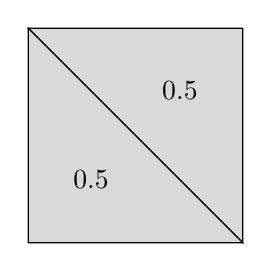
\begin{tikzpicture}[scale=2]
        \hatsinsquare{0.5}
    \end{tikzpicture}
    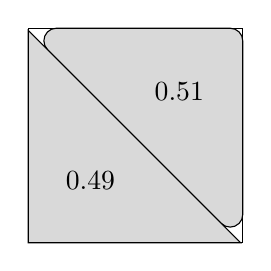
\begin{tikzpicture}[scale=2]
        \hatsinsquare{0.49}
    \end{tikzpicture}
    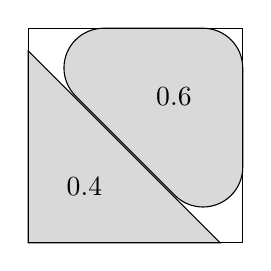
\begin{tikzpicture}[scale=2]
        \hatsinsquare{0.4}
    \end{tikzpicture}
    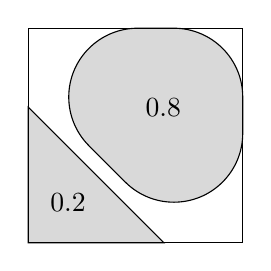
\begin{tikzpicture}[scale=2]
        \hatsinsquare{0.2}
    \end{tikzpicture}
    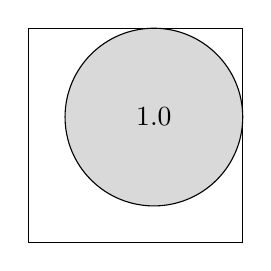
\begin{tikzpicture}[scale=2]
        \hatsinsquare{0}
    \end{tikzpicture}

    \caption{The two shapes' parameters are $(a,b,F)$-conjugated, which is why they always can be packed. The numbers represent $a_1$ and $a_2$, and in this case are the areas of the shapes' incircles.}
    \label{fig:conjugated}
\end{figure}

\section{Split Packing}

The \textsc{Split} algorithm presented in the previous section, in addition to the properties of the instances it produces, are the foundations on which we now build the central theorem of this thesis: The Split Packing theorem. Split Packing by itself is a general approach to pack circles and other shapes into containers. The later chapters of this thesis will all apply the Split Packing theorem to different object and container types.

First, another definition. We will often want to state that a shape can pack all circle instances which belong to a certain class. For this, we define the term \emph{$\mathcal{C}$-shape}:

\begin{definition}
    For any $\mathcal{C} \subseteq \C$, a \emph{$\mathcal{C}$-shape} is a shape in which each $C \in \mathcal{C}$ can be packed.
\end{definition}

For example, if a shape is a $\C(a)$-shape, it means that it can pack all circle instances with a combined area of $a$. And a $\C(a,b)$-shape can pack all circle instances with a combined area of $a$, whose circles each have an area of at most $b$.
With these preparations, we can now state our central theorem:

\begin{theorem}[Split Packing]\label{th:split-packing}
    A shape $s$ is a $\C(a,b)$-shape if there is a split key $F$, so that for all $(a,b,F)$-conjugated tuples $(a_1, b_1)$ and $(a_2, b_2)$ one can find a $\C(a_1, b_1)$-shape and a $\C(a_2, b_2)$-shape which can be packed into $s$.
\end{theorem}

\begin{proof}
    Consider an arbitrary $C \in \C(a,b)$.
    We use \textsc{Split}$(C,F)$ to produce two subinstances $C_1$ and $C_2$. We know from \Cref{th:split-properties} that those subinstances will always be $(a,b,F)$-conjugated. So if we can indeed find two shapes which can pack these subinstances, and if we can pack these two shapes into $s$, then we also can pack the original circle instance $C$ into $s$.

Note that in the extreme case that $C$ consists of a single circle, \textsc{Split}$(C,F)$ will yield two circle instances $C_1 = \{C\}$ and $C_2 = \emptyset$. For this case, \Cref{th:split-properties} guarantees a minimum size of $a$ for the first group, and the associated $\C(a_1,b_1)$-shape is just an $a$-circle. This means that we can simply place the input circle in the container, and stop the recursion at this point.
\end{proof}

Written as an algorithm, Split Packing looks like this:

\begin{algorithm}
    \caption{\textsc{Splitpack}$(s,C)$}
    \begin{algorithmic}
        \Require A $\C(a,b)$-shape $s$ and a circle instance $C \in \C(a,b)$, sorted decendingly by size
        \Ensure A packing of $C$ into $s$
        \State Determine split key $F$ for shape $s$
        \State $(C_1, C_2) \gets \textsc{Split}(C,F)$ \Comment{See \Cref{alg:split}.}
        \ForAll{$i \in \{1,2\}$}
            \State $a_i \gets \mysum(C_i)$
            \State $b_i \gets$ minimum guarantee for $C_i$ \Comment{See \Cref{def:conjugated}.}
            \State Determine a $\C(a_i, b_i)$-shape $s_i$
            \State \Call{Splitpack}{$s_i, C_i$}
        \EndFor
        \State Pack $s_1$, $s_2$, and their contents into $s$
    \end{algorithmic}
\end{algorithm}

To summarize, to apply \textsc{Splitpack} to a shape, we need the following elements:

\begin{enumerate}
    \item A strategy to determine the shape-specific split key $F$.
    \item A strategy to determine a $\C(a_1, b_1)$-shape and a $\C(a_2, b_2)$ for all $(a,b,F)$-conjugated tuples $(a_1, b_1)$ and $(a_2, b_2)$.
    \item A strategy to pack these two shapes into $s$, and a proof why this always works.
\end{enumerate}

Note that the Split Packing algorithm can easily be extended to allow splitting into more than two subgroups. For simplicity, we only describe the case of two subgroups here, as this suffices for the shapes we discuss in this thesis.

\section{Analysis}

There are two perspectives on the implications of the Split Packing theorem. Suppose that we have all three elements mentioned above in place so that we can use Split Packing to pack each circle instance in $\C(a)$ into a given shape.
First, we now have a sufficient condition for the decision problem if a given circle instance can be packed into a given container: If the circles have a combined area of at most $a$, then the instance can be packed.

Second, Split Packing can also be used as an approximation algorithm. Say you are given a circle instance of combined area $a$, but now we want to find the smallest container of a certain shape (for example, triangular or square) in which the instance can be packed. We can then use Split Packing as an approximation algorithm: Select a $\C(a)$-shape whose guaranteed packing density $d$ is as high as possible. We can then be sure that this container has at most $\frac{1}{d}$ times the area of the optimal container.

We will first show that Split Packing has polynomial runtime, as required for an approximation algorithm, and then argue about the approximation factor.

\begin{theorem}
    Split Packing requires $\mathcal{O}(n)$ basic geometric constructions and $\mathcal{O}(n^2)$ numerical operations.
\end{theorem}

\begin{proof}
    To argue why we only need a linear number of geometric constructions, we can count the nodes of the recursion tree: Each subcontainer either has two children (if more than one circle needs to be packed inside, in which case a \textsc{Split} is performed), or one (in this case, the child is a single circle and the recursion ends). Without the circles, the recursion tree is a full binary tree with $n$ leaf nodes, meaning that it has exactly $n-1$ interior nodes. The root node is the container of the packing problem, which does not need to be packed. In total, we need to pack $2n-2$ subcontainers, in addition to the $n$ circles of the input instance, leading to $\mathcal{O}(n)$ geometric constructions.

    In addition, to build the recursion tree, we need at most a quadratic number of numeric operations:
    Before \textsc{Splitpack} is first invoked, the circle instance has to be sorted descendingly by size, this can be done in $\mathcal{O}(n \log n)$ time. Additionally, each run of the \textsc{Split} subroutine then takes linear time in the size of its input. If \textsc{Split} would partition its input into two subinstances with a similar number of elements in each case, this would also lead to a runtime of $\mathcal{O}(n \log n)$, but in the worst case, each run only splits off one element, so that the total time needed for all \textsc{Split} operations is

    $$n + (n-1) + (n-2) + \dots + 1 \in \mathcal{O}(n^2).$$
\end{proof}

\begin{theorem}
    Split Packing, when used to pack circles into a $\C(a,b)$-shape of area $A$, is an approximation algorithm with an approximation factor of $\frac{A}{a}$, compared to the container of minimum area.
\end{theorem}

\begin{proof}
    We know from the previous theorem that Split Packing has polynomial runtime.

    As for the approximation factor, we can be sure that the area of the optimal container $OPT$ needs to be as least $a$, as we need to be able to fit the circles inside without overlap:

    $$OPT \ge a$$

    At the same time, the area of the approximated container $ALG$ is exactly $A$, which means that

    $$\frac{\text{ALG}}{\text{OPT}} \le \frac{A}{a}.$$
\end{proof}

\chapter{Packing circles}\label{ch:circles}

In the previous chapter, we gave a very general description of how Split Packing works. In this chapter, we will show how to apply the approach to concrete packing problems, namely, packing circles into certain triangles and rectangles. For each shape, we will demonstrate two properties: First, we will argue about the \emph{worst-case circle instance} in terms of the density of its optimal packing. This instance constitutes an upper bound to the question “How much area can always be packed?”, because we can show that, given more area, we can find instances which \emph{cannot} be packed.

But second, we are going to show how Split Packing can be used to pack all instances of this area into the shape. This is a constructive way to show a lower bound to our problem. Both pieces together give the answer to \Cref{prb:1}: We have found the largest area $a$, so that circles with this combined area can always be packed into the shape, and we have a polynominal-time algorithm that actually realizes the packing.

\section{Hats}

We saw in \Cref{ch:split-packing} that when applying \textsc{Split} to a circle instance, we can make statements about the minimum circle size of the “relatively larger” group.
If you think about how a circle of minimum size can be placed in a container, there may be certain points which can never be covered by a circle without overlapping the container's boundary. For example, if the container's boundary contains sharp angles, the minimum-size circle may be too large to cover all the angle's area. As we cannot use this for packing the circle instance at all, we may as well cut this area from the container without changing its packing capabilities.

Technically, you can calculate the usable area of a container shape by first eroding it by a circle of minimum size, and then dilating the result with the same circle.

This observation motivates a family of shapes which resemble rounded triangles. We call these shapes \emph{hats}:

\begin{definition}
    For each $0 \le b \le a$, an \emph{$(a,b)$-hat} is a non-acute triangle with an incircle of area $a$, whose corners are rounded to the radius of a $b$-circle, see \Cref{fig:hat}.
    Call the two lower angles of the original triangle \emph{left-angle} and \emph{right-angle}.
    If we say \emph{right hat} or \emph{obtuse hat}, the hat is based on a right/obtuse triangle.
\end{definition}

\newcommand\defaulta{30}
\newcommand\defaultb{40}
\newcommand\defaultr{0.2}
\newcommand\defaultx{0.7}

\fig[3.5]{hat}{An $(a,b)$-hat.}

In the rest of this section, we will show that all circle instances with a combined area of up to $a$ with a minimum circle size of $b$ can be packed into an $(a,b)$-hat.

\begin{definition}\label{def:hat-split-key}
    To get a hat's \emph{associated split key}, split the underlying triangle orthogonally to its base through its tip, and inscribe two circles in the two sides, see \Cref{fig:hat-f}. The areas of these circles are the two components of the hat's split key.
\end{definition}

\fig[3.5]{hat-f}{A hat's \emph{associated split key} equals $(f_1, f_2)$}

To prepare for the next proof, we establish the following lemma:

\begin{lemma}\label{th:overlap}
    Place two circles of combined area $a$ in two corners of a triangle, like in \Cref{fig:hats-overlap}. Let $w$ be the length of the connecting side of the triangle. Now, define $p_1$ and $p_2$ to be the “projection factors”, so that, when projecting circle $a_i$ down onto the connecting side, the distance between the triangle's corner and the far point of the projection is $\sqrt{a_i}p_i$. Note that these factors will be constant for arbitrary circle areas. The two projections do not intersect if

    $$w \ge \sqrt{a(p_1^2 + p_2^2)}.$$
\end{lemma}

\begin{proof}
    Let $w'(a_1) = \sqrt{a_1}p_1 + \sqrt{a-a_1}p_2$ be the combined width of both projections. This function has its global maximum at $a_1 = \frac{p_1^2}{p_1+p_2}a$, and the maximum value is $\sqrt{a(p_1^2+p_2^2)}$. If $w$ is at least as large as this value, the two projections do never intersect.
\end{proof}

\fig[3.5]{hats-overlap}{The circles' projections do not overlap if $w \ge \sqrt{a(p_1^2 + p_2^2)}$.}

\begin{lemma}\label{th:hats-in-hat}
    Consider an $(a,0)$-hat with the associated split key $F = (f_1, f_2)$, and call its left- and right-angles $\alpha$ and $\beta$.
    For all $(a,0,F)$-conjugated tuples $(a_1, b_1)$ and $(a_2, b_2)$, the following two shapes can be packed into the hat:
    \begin{itemize}
        \item A right $(a_1,b_1)$-hat with a right-angle of $\alpha$ and
        \item a right $(a_2,b_2)$-hat with a left-angle of $\beta$.
    \end{itemize}
\end{lemma}

\begin{proof}
    Place the hats' tips at the bottom of the container hat, rotate their $\alpha$- and $\beta$-angles toward the container's matching angles and push them as far to the left/right as possible. \Cref{tab:hats-in-hat} illustrates how these packings looks like for different values of $a_1$ and~$a_2$ and gives some informal reasoning why they can always be packed.

    \begin{table}[p]
        \caption{Hat-in-hat packings for different values of $a_1$ and $a_2$.}
        \label{tab:hats-in-hat}

        \begin{tabular}{cp{7cm}}
            \begin{tikzpicture}[scale=1.8,baseline={([yshift={-\ht\strutbox}]current bounding box.north)},outer sep=0pt,inner sep=0pt]
                \hatsinhat{\defaulta}{\defaultb}{1}{0}
            \end{tikzpicture}
            & When $a_2 = a$, the second hat is simply rounded to a circle of area $a$. By definition, this is the incircle of the container, so it can be packed.\\

            \begin{tikzpicture}[scale=1.8,baseline={([yshift={-\ht\strutbox}]current bounding box.north)},outer sep=0pt,inner sep=0pt]
                \hatsinhat{\defaulta}{\defaultb}{0.9}{0}
            \end{tikzpicture}
            & As $a_2$ gets smaller, the second hat gets less rounded, but still enough so that it can be packed. The other hat is a non-rounded triangle, which fits beside the second one.\\

            \begin{tikzpicture}[scale=1.8,baseline={([yshift={-\ht\strutbox}]current bounding box.north)},outer sep=0pt,inner sep=0pt]
                \hatsinhat{\defaulta}{\defaultb}{0.7}{0}
            \end{tikzpicture}
            & \\

            \begin{tikzpicture}[scale=1.8,baseline={([yshift={-\ht\strutbox}]current bounding box.north)},outer sep=0pt,inner sep=0pt]
                \hatsinhat{\defaulta}{\defaultb}{0.5}{0}
            \end{tikzpicture}
            & \\

            \begin{tikzpicture}[scale=1.8,baseline={([yshift={-\ht\strutbox}]current bounding box.north)},outer sep=0pt,inner sep=0pt]
                \hatsinhat{\defaulta}{\defaultb}{0.43}{0}
            \end{tikzpicture}
            & When $a_1$ and $a_2$ have a ratio as specified by the container's associated split key, the two hats are both non-rounded triangles, but they can still be packed.\\

            \begin{tikzpicture}[scale=1.8,baseline={([yshift={-\ht\strutbox}]current bounding box.north)},outer sep=0pt,inner sep=0pt]
                \hatsinhat{\defaulta}{\defaultb}{0.3}{0}
            \end{tikzpicture}
            & When $a_2$ gets smaller than specified by the split key, it is now the first container which is getting more rounded.\\

            \begin{tikzpicture}[scale=1.8,baseline={([yshift={-\ht\strutbox}]current bounding box.north)},outer sep=0pt,inner sep=0pt]
                \hatsinhat{\defaulta}{\defaultb}{0.1}{0}
            \end{tikzpicture}
            & As $a_1$ approaches $a$, it is now the first hat whose shape gets closer to a perfect $a$-circle.\\

            \begin{tikzpicture}[scale=1.8,baseline={([yshift={-\ht\strutbox}]current bounding box.north)},outer sep=0pt,inner sep=0pt]
                \hatsinhat{\defaulta}{\defaultb}{0}{0}
            \end{tikzpicture}
            & By the same argument as before, this circle can be packed.\\
        \end{tabular}
    \end{table}

    This way of placing the two hats results in a valid packing if (1) the hats do not overlap each other and (2) the hats fit into the hat individually. We are going to proof these two properties separately.

    We first want to show that the hats do not overlap each other. If the hats' projections onto the container's base do not overlap, we found a separating axis and can be sure that the hats do not overlap, as well. Furthermore, because the hats' incircles touch the rightmost part of the left hat's boundary and the leftmost part of the right hat's boundary, it suffices to show that the projections of the hats' incircles onto the container's base do not overlap.

    We want to use \Cref{th:overlap} for this proof, so we need to make a statement about the projection factors $p_1$ and $p_2$ in \Cref{fig:hatlr}: If the top angle is a right angle, we can see that $\sqrt{a}p_1 = x$ and $\sqrt{a}p_2 = y$. So by the Pythagorean theorem, $w^2 = (\sqrt{a}p_1)^2 + (\sqrt{a}p_2)^2$.
     If the top angle is more obtuse, but the incircle's center stays at the same $x$-coordinate (like the dotted variant in \Cref{fig:hatlr}),
    both $\sqrt{a}p_1$ and $\sqrt{a}p_2$ only get smaller, so for each hat, $w^2 \ge (\sqrt{a}p_1)^2 + (\sqrt{a}p_2)^2$, which is equivalent to $w \ge \sqrt{a(p_1^2+p_2^2)}$.
    By \Cref{th:overlap}, this means that the projections of the circles do not overlap, which in turn means that the two hats do not overlap.

    \fig[4]{hatlr}{$l^2 + r^2 \le 1$ holds for each non-acute triangle}

    The second property we need to show is that the hats fit into the container individually. Unfortunately, this part of the proof is going to be long and technical.

    If a hat's incircle is not larger than the incircle of the container hat's side, it will fit into the container without question because it is a subset of that side (like all the non-rounded hats in \Cref{tab:hats-in-hat}).
    So let us assume $a_i > f_i$.

    In this proof, we are going to use two different length-area ratios, which are illustrated in \Cref{fig:hat-poke-f}. The first one is $d$, which describes the ratio between the length of the triangle's right leg and the square root of the area of its right incircle $f_i$. Note that for all triangles \emph{similar} to the right part of the container triangle, this ratio between the length of this edge and the square root of the incircle's area will be constant.
    The second ratio, $e$, is the ratio between the length of the same right leg and the square root of the incircle-area of the whole container triangle. Again, it is a constant for triangles similar to the given container triangle. Note that, in preparation for a generalization later in this chapter, we denote the triangle's incircle by $o$.
    From \Cref{fig:hat-poke-f} we can now observe that
    $e\sqrt{o} = d\sqrt{f_i}$, which is equivalent to $e = d\sqrt{f_i/o}$.

    \fig[3.5]{hat-poke-f}{The ratios $d$ and $e$ are constant for all similar triangles.}


    Moving forward, in \Cref{fig:hat-poke}, we display the situation when packing a hat into (\wlofg) the right leg of the container. $f_i$ is the relevant factor from the split key, $a_i$ is the hat's incircle and $b_i$ represents the hat's rounding.

    \fig[3.5]{hat-poke}{Various measurements when packing a rounded hat.}

    The hat is placed in such a way that it will never overlap the bottom or the right leg of the containing triangle, so it is sufficient to show that it does not overlap the left leg.
    We can tell from \Cref{fig:hat-poke} that this does not happen if the length of the right side of the triangle the hat is based on ($d\sqrt{a_i}$), minus the length of the right side of the $(b_i,0)$-triangle similar to the containers right side ($d\sqrt{b_i}$), plus the length of the right side of the $(b_i,0)$-triangle similar to the container ($e\sqrt{b_i}$) is at most the length of the container's right leg ($d\sqrt{f_i}$). So the following condition has to hold:

    \begin{equation*}
        d\sqrt{a_i} - d\sqrt{b_i} + e\sqrt{b_i} \le d\sqrt{f_i}
    \end{equation*}

    As previously observed, $e = d\sqrt{f_i/o}$:

    \begin{equation*}
        d\sqrt{a_i} - d\sqrt{b_i} + d\sqrt{f_i/o}\sqrt{b_i} \le d\sqrt{f_i}
    \end{equation*}

    In our case, the incircle of the triangle has exactly the maximal area which we want to pack, so $o = a$. But even if $o \ge a$, the inequality is true if

    \begin{equation*}
        d\sqrt{a_i} - d\sqrt{b_i} + d\sqrt{f_i/a}\sqrt{b_i} \le d\sqrt{f_i}
    \end{equation*}

    We can also divide by $d$ and factor out $\sqrt{b_i}$ to get:

    \begin{equation}\label{eq:tripoke}
        \sqrt{a_i} - (1-\sqrt{f_i/a})\sqrt{b_i} \le \sqrt{f_i}
    \end{equation}


    Let $j$ be the index of the other hat to be packed.
    We know (from the conjugatedness) that the sum of both hats' incircles does not exceed the total area $a$, so $a_i + a_j \le a$. Also, $f_i + f_j \ge a$, as demonstrated in \Cref{fig:hat-f-sum}: In right triangles, $f_1 + f_2$ is exactly $a$, because as its two halves are \emph{similar} to the large triangle, the two halves' areas add up to the container triangle's area, and the ratio between the areas of a triangle and its incircle are constant. When making the upper angle more obtuse, but letting $f_1$ and $f_2$ stay the same, the incircle only shrinks (like the dotted variant in \Cref{fig:hat-f-sum}).

    \fig[4]{hat-f-sum}{In non-acute triangles, $f_1 + f_2 \ge a$.}

    Putting it together, by \Cref{th:split-properties}, our hat it is rounded by

    $$b_i \ge a_i - f_i\frac{a_j}{f_j} \ge a_i - f_i\frac{a-a_i}{a-f_i} = \frac{a_i(a-f_i)-f_i(a-a_i)}{a-f_i} = a\frac{a_i-f_i}{a-f_i}$$

    Insert that into \Cref{eq:tripoke}:

    $$\sqrt{a_i} - (1-\sqrt{f_i/a})\sqrt{a\frac{a_i-f_i}{a-f_i}} \le \sqrt{f_i}$$

    Then bring the subtrahend to the right and square both sides (both are positive):

    $$a_i \le f_i + 2\sqrt{f_i}(1-\sqrt{f_i/a})\sqrt{a\frac{a_i-f_i}{a-f_i}} + (1-\sqrt{f_i/a})^2a\frac{(a_i-f_i)}{a-f_i}$$

    Subtract $f_i$ and divide by $\sqrt{a_i-f_i}$:

    $$\sqrt{a_i-f_i} \le \frac{2\sqrt{f_i}(1-\sqrt{f_i/a})\sqrt{a}}{\sqrt{a-f_i}} + (1-\sqrt{f_i/a})^2a\frac{\sqrt{a_i-f_i}}{a-f_i}$$

    Rearrange:

    $$\sqrt{a_i-f_i}\frac{(a-f_i)-(1-\sqrt{f_i/a})^2a}{a-f_i} \le \frac{2\sqrt{f_i}(1-\sqrt{f_i/a})\sqrt{a}}{\sqrt{a-f_i}}$$

    Simplify:

    $$\sqrt{a_i-f_i}\frac{2\sqrt{f_ia}-2f_i}{a-f_i} \le \frac{2\sqrt{f_ia}-2f_i}{\sqrt{a-f_i}}$$

    Then multiply with $\sqrt{a-f_i}$:

    $$\sqrt{a_i-f_i}\frac{2\sqrt{f_ia}-2f_i}{\sqrt{a-f_i}} \le \frac{2\sqrt{f_ia}-2f_i}{\sqrt{a-f_i}}\sqrt{a-f_i}$$

    Finally, divide by the fraction to get:

    \begin{equation*}
        \sqrt{a_i-f_i} \le \sqrt{a-f_i} \iff a_i - f_i \le a - f_i \iff a_i \le a
    \end{equation*}

    From the conjugatedness we know that $a_i$ is never larger than $a$, so \Cref{eq:tripoke} is true and the hat always fits into the container. This completes the proof of \Cref{th:hats-in-hat}.
\end{proof}

Until now, the container was always an $(a,0)$-hat, which is essentially a non-rounded triangle with an incircle of $a$. The next lemma extends this idea to hats which are actually rounded. It is identical to \Cref{th:hats-in-hat}, except that the rounding of the container hat is no longer 0, but $b$.

\begin{lemma}\label{th:rounded-hats-in-hat}
    Consider an $(a,b)$-hat with the associated split key $F = (f_1, f_2)$, and call its left- and right-angles $\alpha$ and $\beta$.
    For all $(a,b,F)$-rounded tuples $(a_1, b_1)$ and $(a_2, b_2)$ with $a_1 + a_2 \le a$, the following two shapes can be packed into the hat:
    \begin{itemize}
        \item A right $(a_1,b_1)$-hat with a right-angle of $\alpha$ and
        \item a right $(a_2,b_2)$-hat with a left-angle of $\beta$.
    \end{itemize}
\end{lemma}

\begin{proof}
    \Cref{th:hats-in-hat} tells us that this theorem is true for $b = 0$. Now, the container's corners can be rounded to the radius of a $b$-circle, and we need to show that the two hats from the previous construction still fit inside. But all of the two hat's corners are also rounded to (at least) the same radius (see \Cref{th:split-properties}), so they will never overlap the container, see \Cref{fig:hats-rounding}.
\end{proof}

\fig[2.5]{hats-rounding}{Rounding all hats' corners by the same radius does not affect the packing.}

With these preparations, we can finally apply Split Packing to hats:

\begin{theorem}\label{th:hats}
    Given an $(a,b)$-hat, all circle instances with a combined area of at most $a$ and a minimum circle size of at least $b$ can be packed into that triangle.
\end{theorem}

\begin{proof}
    We proof by induction that we can pack each $C \in \C(a,b)$ into the hat:

    If $C$ only consists of a single circle, it can be packed into the hat, as it is at most as big as the hat's incircle.

    Now assume that for any $0 \le b \le a$, any $(a,b)$-hat could pack all circle instances into $\C(a,b)$ with at most $n$ circles. Consider a circle instance $C \in \C(a,b)$ containing $n+1$ circles.
    \Cref{def:hat-split-key} tells us how to compute the split key $F$.
    Then we know from \Cref{th:split-properties} that \textsc{Split} will partition $C$ into two subinstances $C_1 \in \C(a_1, b_1)$ and $C_2 \in \C(a_2, b_2)$, whose parameters are $(a,b,F)$-rounded. As \textsc{Split} can never return an empty instance (except for $|C| = 1$, a case which we handled above), each subinstance will contain at most $n$ circles. We know from \Cref{th:rounded-hats-in-hat} that, for all pairs of $(a,b,F)$-rounded tuples, we can find two hats with matching parameters which fit into the container hat. By assumption, these hats can now pack all instances from $\C(a_1, b_1)$ and $\C(a_2, b_2)$, respectively, which means that they can especially also pack $C_1$ and $C_2$. If we then pack the two hats into the container, we have constructed a packing of $C$ into the container hat.

    By induction, we can pack each $C \in \C(a,b)$ into the $(a,b)$-hat.
\end{proof}

\pagebreak

\section{Non-acute triangles}

As a non-acute triangles is only a special case of a hat, this section is will be pleasantly short.

\begin{theorem}\label{th:tri}
    Given a non-acute triangle with an incircle of area $a$, all circle instances with a combined area of up to $a$ can be packed into the triangle, and this bound is tight.
    See \Cref{fig:example-circles-in-right} for some example packings.
    Expressed algebraically, for a triangle with side lengths $a$, $b$, and $c$, the critical density is

    $$\sqrt{\dfrac{-(a-b-c)(a+b-c)(a-b+c)}{(a+b+c)^3}}\pi < 53.91\%.$$
\end{theorem}

\begin{proof}
    The triangle is an $(a,0)$-hat, which by \Cref{th:hats} is a $\C(a)$-shape.

    On the other hand, a single circle of area $a + \varepsilon$ cannot be packed, as the incircle is by definition the largest circle which fits into the triangle.

    As for the algebraic formulation of the critical density, the area of the triangle can be calculated using Heron's formula:

    $$\Delta(a,b,c) := \sqrt{s(s-a)(s-b)(s-c)} \text{ with } s = \frac{a+b+c}{2}$$

    It is also known that the radius of the incircle of this triangle is

    $$R(a,b,c) := \frac{\Delta(a,b,c)}{s} \text{ with } s = \frac{a+b+c}{2},$$

    so the incircle has an area of

    $$I(a,b,c) = \pi R(a,b,c)^2 = \frac{(a+b-c)(c+a-b)(b+c-a)}{4(a+b+c)}.$$

    Finally, the ratio between the areas of the circle and the triangle can be calculated to be

    $$\frac{I(a,b,c)}{\Delta(a,b,c)} = \sqrt{\dfrac{-(a-b-c)(a+b-c)(a-b+c)}{(a+b+c)^3}}\pi.$$
\end{proof}

\begin{figure}[p]
    \begin{tabular}{cc}
        \subfig[0.013]{example-circles-in-right-1} &
        \subfig[0.013]{example-circles-in-right-2} \\
        \subfig[0.013]{example-circles-in-right-3} &
        \subfig[0.013]{example-circles-in-right-4} \\
        \subfig[0.013]{example-circles-in-right-5} &
        \subfig[0.013]{example-circles-in-right-6} \\
    \end{tabular}
    \caption{Example packings of various circle instances into a right triangle produced by Split Packing.}
    \label{fig:example-circles-in-right}
\end{figure}

\section{Isosceles triangles}

Split Packing can pack with critical density not only into non-acute triangles, but also into isosceles triangles, as long as its two symmetric sides are not longer than the base. In this sense, it works for all triangles inbetween a right isosceles triangle and an equilateral triangle.

\begin{definition}
    A \emph{thick isosceles triangle} is an isosceles triangle whose legs are at most as long as its base, but whose top angle is at least $\frac{\pi}{4}$. Examples are shown in \Cref{fig:iso-range}.
\end{definition}

\fig[1]{iso-range}{Range of considered isosceles triangles.}

To prove the worst case for these triangles, we first make a statement about a triangle's \emph{twincircles}:

\begin{lemma}\label{th:iso-worst}
    Two touching equal circles, placed in the corners connected by a triangle's longest side, are the triangle's twincircles, meaning there are no two larger equal circles which can be packed.
\end{lemma}

\begin{proof}
    Call the circles' radius $r$.
    When eroding the triangle by $r$, the remaining area is a triangle similar to the original one, whose longest side has a length of $2r$, see \Cref{fig:twincircles-construction}. This means that when eroding the triangle by $r+\varepsilon$, the longest side of the remaining area must be shorter than $2r$.
    But to pack two circles with radius $r+\varepsilon$, their centers need to be placed at least $r+\varepsilon$ away from the triangle's boundary and at least $2r+2\varepsilon$ away from each other. The construction shows that this is not possible.
\end{proof}

\fig{twincircles-construction}{Two circles larger than these cannot be packed.}

In the previous section, the target area $a$ which we wanted to pack always was the area of the triangles incircle. For thick isosceles triangles, the twincircle area, is \emph{smaller} than the incircle area, which means it will not always be possible to pack the area of the incircle.
In this section, we will argue that we can always pack the twincircle area into thick isosceles triangles.

\begin{definition}
    The split key of a thick isosceles triangle is $(1,1)$.
\end{definition}

\begin{lemma}\label{th:hats-in-iso}
    Consider a thick isosceles triangle with a twincircle area of $a$ and call its symmetric angles $\alpha$.
    For all $(a,0,(1,1))$-conjugated tuples $(a_1, b_1)$ and $(a_2, b_2)$, the following two shapes can be packed into the hat:
    \begin{itemize}
        \item A right $(a_1,b_1)$-hat with a right-angle of $\alpha$ and
        \item a right $(a_2,b_2)$-hat with a left-angle of $\alpha$.
    \end{itemize}
\end{lemma}

\begin{proof}
    See \Cref{fig:hats-in-iso} for example packings for different $a_1$ and $a_2$.

    First, we show that the hats do not intersect each other: In any isosceles triangle, the projection factors for both sides, $p_1$ and $p_2$ are equal. So in \Cref{fig:iso-width}, we construct the width of the triangle's base to be $2\sqrt{\frac{a}{2}}p_1 = \sqrt{2ap_1^2} = \sqrt{a(p_1^2+p_2^2)}$. By \Cref{th:overlap}, this means that the hats do not overlap.

    \fig{iso-width}{The width of an isosceles triangle is $\sqrt{2ap_1^2}$.}

    Second, we show that the hats do not intersect the container. We are going to re-use the proof from \Cref{th:hats-in-hat} here. On \cpageref{eq:tripoke}, we showed that the hats do not overlap the container if certain conditions are met. These conditions are also true here:

    \begin{itemize}
        \item $a_1 + a_2 \le a$, the hat's incircles add up to at most $a$ because of the conjugatedness of the tuples.
        \item $f_i + f_j \ge a$, in this case, the incircle-areas of the triangles sides are equal to $a$ by assumption.
        \item $o \ge a$, meaning that the triangles incircle is at least as large as the area of the twincircles. This can be demonstrated like in \Cref{fig:hat-f-sum} on \cpageref{fig:hat-f-sum}, but in the reverse direction: For a right isosceles triangle, the twincircle area $a$ is exactly equal to the triangle's incircle. If leaving the twincircles in place, but increasing the top angle, the incircle only gets larger.
    \end{itemize}

    So also in this case, the hats do not overlap the container. This concludes the proof.
\end{proof}

\begin{figure}
    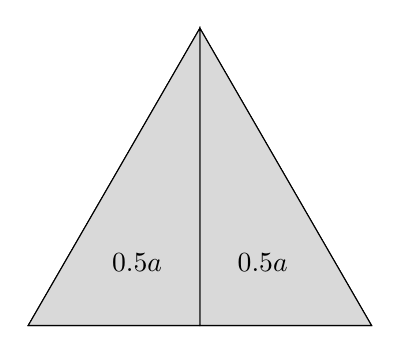
\begin{tikzpicture}[scale=2]
        \hatsinhat[1.244]{60}{60}{0.5}{0}
    \end{tikzpicture}
    ~
    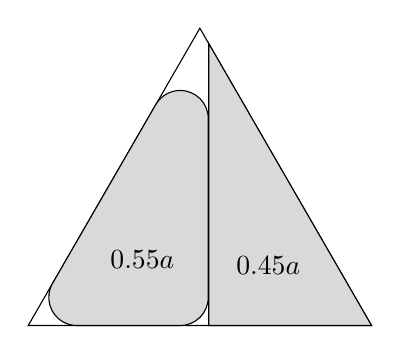
\begin{tikzpicture}[scale=2]
        \hatsinhat[1.244]{60}{60}{0.45}{0}
    \end{tikzpicture}
    ~
    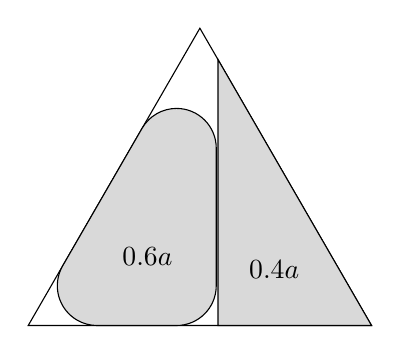
\begin{tikzpicture}[scale=2]
        \hatsinhat[1.244]{60}{60}{0.4}{0}
    \end{tikzpicture}

    \vspace{10pt}

    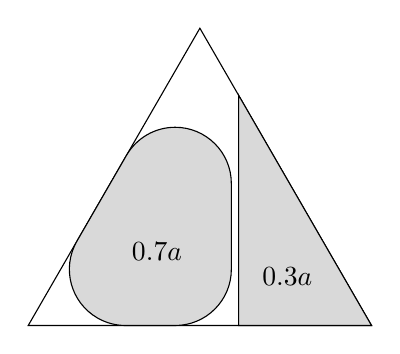
\begin{tikzpicture}[scale=2pt]
        \hatsinhat[1.244]{60}{60}{0.3}{0}
    \end{tikzpicture}
    ~
    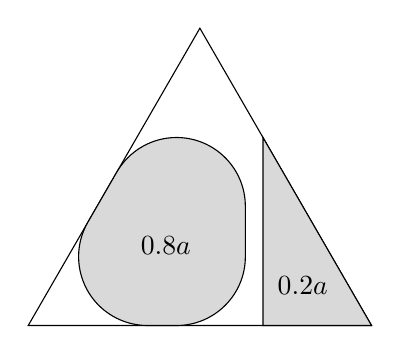
\begin{tikzpicture}[scale=2pt]
        \hatsinhat[1.244]{60}{60}{0.2}{0}
    \end{tikzpicture}
    ~
    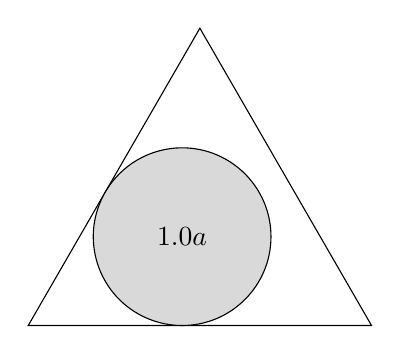
\begin{tikzpicture}[scale=2]
        \hatsinhat[1.244]{60}{60}{0}{0}
    \end{tikzpicture}

    \caption{Packing two hats into an equilateral triangle.}
    \label{fig:hats-in-iso}
\end{figure}

\begin{theorem}\label{th:iso}
    Given a thick isosceles triangle with a twincircle area of $a$, all circle instances with a combined area of up to $a$ can be packed into the triangle, and this area bound is tight.
    See \Cref{fig:example-circles-in-equilateral} for some example packings.
    Expressed algebraically, for a triangle with legs of length $b$ and a base of length $c$, the critical density is

    $$48.60\% < \frac{(c-2b+\sqrt{4b^2-c^2})^2\pi}{2c\sqrt{4b^2-c^2}} < 53.91\%$$
\end{theorem}

\begin{proof}
    By \Cref{th:hats-in-iso} and the Split Packing Theorem, the triangle is a $\C(a)$-shape.

    In \Cref{th:iso-worst}, we argued that any two equal circles larger than the twincircles cannot be packed.

    We use Heron's formula again to calculate a critical density of

    $$\frac{2I(\frac{c}{2}, b, h)}{\frac{c}{2}h} = \frac{(c-2b+\sqrt{4b^2-c^2})^2\pi}{2c\sqrt{4b^2-c^2}}.$$
\end{proof}

\begin{figure}[p]
    \begin{tabular}{cc}
        \subfig[0.015]{example-circles-in-equilateral-1} &
        \subfig[0.015]{example-circles-in-equilateral-2} \\
        \subfig[0.015]{example-circles-in-equilateral-3} &
        \subfig[0.015]{example-circles-in-equilateral-4} \\
        \subfig[0.015]{example-circles-in-equilateral-5} &
        \subfig[0.015]{example-circles-in-equilateral-6} \\
    \end{tabular}
    \caption{Example packings of various circle instances into an equilateral triangle produced by Split Packing.}
    \label{fig:example-circles-in-equilateral}
\end{figure}

\section{The problem with acute triangles}\label{sec:acute-triangles}

A class of triangles for which we could not prove the critical density are general acute triangles. The problem is that the condition for \Cref{th:overlap} is not met, which means that the two hats may overlap:

\fig[3.5]{overlap}{For general acute triangles, the two hats may overlap.}

We worked on the following assumption:

\begin{conjecture}
    A circle instance can be packed into a triangle if the circles' combined area does not exceed the triangles incircle or twincircle, whichever is smaller.
\end{conjecture}

If this conjecture is true, surely there are strategies which can pack into acute triangles with critical density. For example, we attempted to split the circle instance into four subinstances using a slightly modified \textsc{Split} algorithm, and then to pack four hats into the container, like in \Cref{fig:four}. Again, this is motivated by the observation that, when splitting each circle top-down into four equal circles, this strategy always works because the triangle is recursively divided into four similar triangles.

\fig[3.5]{four}{Packing four hats into an acute triangle.}

Unfortunately, this strategy fails for some instances, like depicted in \Cref{fig:four-fail}. For this instance, the largest group, consisting of a single circle, cannot be packed if \emph{any} of the smaller groups is packed into the top or the left corner, because the remaining free space is not wide enough for the circle. Other strategies or a case distinction would need to be considered.

\fig[4]{four-fail}{This strategy does not work for a container with a right-angle of $\frac{\pi}{10}$, incircle $1$ and the circle instance $\{0.55,0.15,0.15,0.15\}$.}

\section{Rectangles}\label{sec:rectangles}

Some of our main results concern the packing of circles into a square. We will cover that packing problem in the next chapter, along with some generalizations on the objects which are to be packed, which is why we do not repeat it here. Instead, we first turn toward rectangles.

Split Packing can be used to pack circles with critical density into rectangles. The basic idea is to divide the rectangle along a diagonal, and pack the subinstances produced by \textsc{Split} into these two halves. If one group gets larger than half, it gets rounded enough so that it sill works. The basic idea is to divide the rectangle along a diagonal, and pack the subinstances produced by \textsc{Split} into these two halves. If one group gets larger than half, it gets rounded enough so that it sill works.

%TODO fix
\begin{figure}
    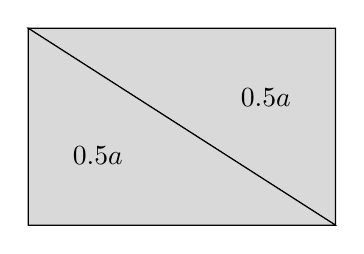
\begin{tikzpicture}[scale=2.5]
        \hatsinrect{0.5}
    \end{tikzpicture}
    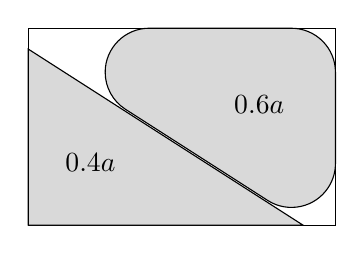
\begin{tikzpicture}[scale=2.5]
        \hatsinrect{0.4}
    \end{tikzpicture}
    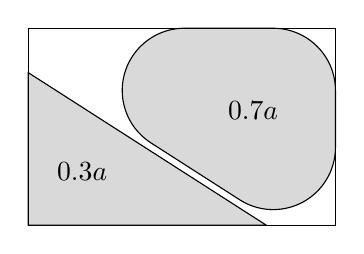
\begin{tikzpicture}[scale=2.5]
        \hatsinrect{0.3}
    \end{tikzpicture}

    \vspace{5mm}

    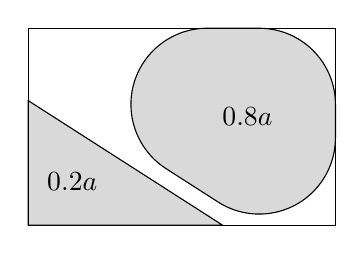
\begin{tikzpicture}[scale=2.5]
        \hatsinrect{0.2}
    \end{tikzpicture}
    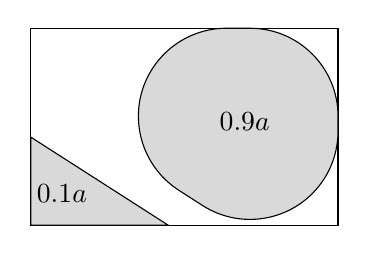
\begin{tikzpicture}[scale=2.5]
        \hatsinrect{0.1}
    \end{tikzpicture}
    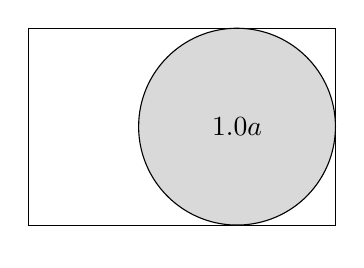
\begin{tikzpicture}[scale=2.5]
        \hatsinrect{0}
    \end{tikzpicture}

    \caption{Hat-in-rectangle packings for different values of $a_1$ and $a_2$.}
    \label{fig:hats-in-rect}
\end{figure}

At this point, we do not know how to handle \emph{all} rectangles, and this has to do with the different classes of worst-cases which appear when packing circles into rectangles of different ratios. \Cref{fig:long-rects} shows several examples. At the top, we show the conjectured worst-case instance. For squares, we already discussed the worst case---it consists of the square's twincircles, the two largest circles which can be packed into the square.

\fig[2.4]{long-rects}{Rectangles of different aspect ratios. Top: Their conjectured worst-case instances. Bottom: The incircles of their halves. Aspect ratios between 1 and $\approx 1.5607$ are the only ones where the area of the worst-case instance is larger than the area of the two circles inscribed in the halves.}

For rectangles with a slightly larger aspect ratio (like 1:1.3), we conjecture that the worst-case instance still consists of the rectangle's twincircles, but we do not know how to pack this area using Split Packing, because when cutting the rectangle along the circles' tangent, the resulting pieces are not triangular. At this point, we do not know how to deal with these kinds of quadrilaterals recursively.

As the aspect ratio gets even larger, at some point the twincircle area gets larger than the incircle of the rectangle, whose diameter is as long as the rectangle's smaller side. Obviously, any circle larger than this incircle cannot be packed, so from this point forward, the worst-case instance of these “long” rectangles will be their incircles.

At the bottom of \Cref{fig:long-rects}, we divided all rectangles along their diagonal, and inscribed circles into the resulting halves. We will show that we can pack circles with critical density into a rectangle if the area of those two circles is at least as large as the worst-case area:
We know from the previous sections that we can pack right hats with incircle density. It is left to show that, if one of the two hats should get larger than the other one, they both can still be packed.

What is the aspect ratio of the rectangle where the combined area of the two circles incribed in the halves is exactly equal to the incircle area? In \Cref{fig:rect-construction}, we see that the area of the incircle is $A = \pi(\frac{h}{2})^2$.

\fig[5]{rect-construction}{Constructing the case where $A = 2B$.}

The proof of \Cref{th:tri} on \cpageref{th:tri} discusses how to use Heron's formula to algebraically find the area of a triangle, given its side lengths.
In our case, $A = 2B$ is equivalent to

$$\frac{\pi}{4}h^2 = 2I(h,w,\sqrt{h^2+w^2}) = \frac{\pi aw(h+w-\sqrt{h^2+w^2}}{h+w+\sqrt{h^2+w^2}}$$

and this equation this is true for $w = \frac{2+3\s}{4}h \approx 1.5607h$.
This means that all rectangles whose side ratio is at least this large can be packed with critical density, simply by using the split key $F = (1,1)$ and by placing two right hats in the rectangle.

\begin{lemma}\label{th:hats-in-rect}
    Consider a rectangle whose longer side $w$ is at least $\frac{2+3\s}{4} \approx 1.5607$ times as long as its shorter side $h$ and let $a$ be the area of its incircle.
    Any two $(a,0,(1,1))$-conjugated right hats similar to the two halves of the rectangle when cutting diagonally from corner to corner can be packed into the rectangle.
\end{lemma}

\begin{proof}
    See \Cref{fig:hats-in-rect} for some example packings. The proof works analogously to the proof of \Cref{th:hats-in-hat}.
\end{proof}

\begin{theorem}\label{th:rect}
    Given a rectangle whose longer side $w$ is at least $\frac{2+3\s}{4} \approx 1.5607$ times as long as its shorter side $h$, let $a$ be the area of its incircle.
    All circle instances with a combined area of up to $a$ can be packed into the rectangle, and this area bound is tight.
    See \Cref{fig:example-circles-in-rect} for some example packings.
    Expressed algebraically, the critical density is $\frac{\pi h}{4w}$.
\end{theorem}

\begin{figure}
    \begin{tabular}{cc}
        \subfig[0.015]{example-circles-in-rect-1} &
        \subfig[0.015]{example-circles-in-rect-2} \\
        \subfig[0.015]{example-circles-in-rect-3} &
        \subfig[0.015]{example-circles-in-rect-4} \\
        \subfig[0.015]{example-circles-in-rect-5} &
        \subfig[0.015]{example-circles-in-rect-6} \\
    \end{tabular}
    \caption{Example packings of various circle instances in a rectangle with aspect ratio 1:1.57 produced by Split Packing.}
    \label{fig:example-circles-in-rect}
\end{figure}

\begin{proof}
    By \Cref{th:hats-in-rect} and the Split Packing Theorem, the rectangle is a $\C(a)$-shape.

    The $a$-circle's diameter is equal to the rectangle's smaller side, so it is clear that any larger circles cannot be packed.

    The critical density is the ratio of the circle's and the rectangle's area, which can be calculated to be $$\frac{\pi (\frac{h}{2})^2}{wh} = \frac{\pi h}{4w} < 50.33\%.$$
\end{proof}

\chapter{Packing rubies}\label{ch:rubies}

In the previous chapter, we showed how Split Packing can be used to pack circular objects into triangles and rectangles.
As we explored generalizations of Split Packing during the creation of this thesis, we usually tried to find additional container shapes for which we could use Split Packing to pack circles with up to critical density. 

But at one point, we decided to try whether we could vary the “other half” of packing problems: The objects. We rarely had thought of packing objects other than circles.\footnote{After all, the preliminary title of this thesis was \emph{Circle Packing Algorithms}!} 
We were surprised to find out that, when we allowed to rotate objects, we could also use Split Packing to pack squares into a square container with up to critical density! Shortly after, we discovered that we could also use it to pack octagons with up to critical density. Both modified packing problems could be solved with only a very small modification of the algorithm.

As we know now, the reason why we can pack circles, squares, as well as octagons, is that all these shapes are subsets of the very special shape shown in \Cref{fig:ruby-intro}. We call this shape \emph{ruby}, because it looks like a cut gemstone from the side:

\fig{ruby-intro}{The “ruby” shape and its contained circle, square and hexagon.}

In this chapter, we will show how to pack rubies into squares and isosceles right triangles with up to critical density. As corollaries, we get critical-density packing algorithms for circles, squares, and octagons for these containers for free!
In fact it turns out that, if you are given a set of objects, no matter what their shape is, if you can enclose them in rubies so that the combined area of the rubies does not exceed the critical density, then you can pack the shapes into these containers.

\section{Gems and rubies}

For this generalization, we need another new shape, which has a similar function as previous chapter's \emph{hats}. Our ruby shape has a very distinct way its corners are cut off. We generalize this cutoff to get to a family of shapes which we call \emph{gems}\footnote{A ruby is a special gem, get it?}:

\begin{definition}
    For each $0 \le b \le a$, an \emph{$(a,b)$-gem} is an isosceles right triangle with an incircle of area $a$, whose acute corners are cut off like shown in \Cref{fig:gem}: Each cut forms an angle of $\frac3 4\pi$ with the triangle's boundary, and the distance of each cut to the triangle's original corner is

    $$c(b) := \frac{(2+\s)(2\sqrt{\s-1}-1)}{\sqrt{2(\s-1)\pi}}\sqrt{b} \approx 0.6078 \sqrt{b}.$$

\end{definition}

\fig[4]{gem}{An $(a,b)$-gem.}

\begin{definition}
    A gem's associated split key is $(1,1)$, as usual for symmetric shapes.
\end{definition}

For the following proofs, we need to know a gem's dimensions in detail.
Consider an ($a,b$)-gem and let $r = \sqrt{\frac{a}{\pi}}$ be the radius of its incircle. By construction in \Cref{fig:gem-construction}, the hat has
\begin{itemize}
    \item cut-width $c(b) = \frac{(2+\s)(2\sqrt{\s-1}-1)}{\sqrt{2(\s-1)\pi}}\sqrt{b}$ (by definition),
    \item diagonal $D(a) = \s(\textcolor{blue}{r\s+r}) = (2+\s)\sqrt{\frac{a}{\pi}}$,
    \item width $w(a,b) = 2(\textcolor{blue}{r\s+r}) - 2c(b) = (2+2\s)\sqrt{\frac{a}{\pi}} - 2c(b)$, and
    \item corner-width $W(a,b) = (2+2\s)\sqrt{\frac{a}{\pi}} - c(b)$.
\end{itemize}

\fig[4]{gem-construction}{Dimensions of an $(a,b)$-gem.}

The definition of a gem is designed so that we get our ruby shape exactly for $a = b$:

\begin{definition}
    We call an $(a,a)$-gem an \emph{$a$-ruby}.
\end{definition}

An $a$-ruby contains the following shapes, see \Cref{fig:gem}:

\begin{itemize}
    \item A circle of area $a$,
    \item a square of area $\frac{3+2\s}{2\pi}a \approx 0.9276a$, and
    \item a regular octagon of area $\frac{8\s-8}{\pi}a \approx 1.0548a$.
\end{itemize}

This is because if the circle's radius is $r = \sqrt{\frac{a}{\pi}}$, then the square has an edge length of $(1+\frac{1}{\s})r$, so its area is $(1+\s+\frac{1}{2})r^2$. Regular $n$-gons with an apothem\footnote{The apothem is the distance of the polygon's center to its sides.} of $r$ have an area of $nr^2\tan(\frac{\pi}{n})$, which, for $n=8$, amounts to $8r^2(\s-1)$.

\fig{ruby}{An $a$-ruby and its contained circle, square and hexagon.}

A ruby itself can be calculated to have an area of $\frac{8\sqrt{2(7+5\s)}-3(7+4\s)}{\pi}a \approx 1.4225a$.

We will also use a modified version of gems and rubies for which only one corner is cut off. We will call these gems \emph{sharp}:

\begin{definition}
    A \emph{sharp $(a,b)$-gem} is an isosceles triangle where only one corner is cut off like in the definition of a gem, see \Cref{fig:sharp-ruby}. A \emph{sharp ruby} is a sharp $(a,a)$-gem.
\end{definition}

\fig[4]{sharp-ruby}{A \emph{sharp} ruby.}

A sharp ruby is a superset of a regular ruby with the same parameters and can be calculated to have an area of $\frac{4\sqrt{2(7+5\s)}-5\s-9}{\pi}a \approx 1.6388a$.

From this point forward, we will no longer pack circles, but (regular and sharp) rubies. To simplify talking about these instances, we make the following definition:

\begin{definition}
    A \emph{ruby instance} is defined excactly like a circle instance (see \Cref{def:circle-instance}), except that the real numbers now define the areas of the rubies' incircles. $\R$ is the set of all ruby instances, $\R(a,b)$ is defined analogously.
    Similarly, we call the set of all \emph{sharp ruby instances} $\myS$, and define $\myS(a,b)$ analogously.
\end{definition}

One way to think about ruby instances is that they consist of the rubies “built around” the circles of a circle instance.

\begin{lemma}\label{th:gems-in-gem}
    Any two $(a, 0, (1,1))$-conjugated sharp gems can be packed into a sharp $(a,0)$-gem.
\end{lemma}

\begin{proof}
    Assume \wlofg\ that the two gems are a sharp $(a_1, b_1)$-gem and a sharp $(a_2, b_2)$-gem with $a_1 \ge a_2$, meaning that we always swap the larger gem to the left. Also, let us normalize $a$ to 1 to make calculations easier. The proofs hold for all $a$, one just needs to multiply all areas with $a$ and all lengths with $\sqrt{a}$.

    Again, we will show that we can always place the gems so that (1) they do not overlap each other and (2) they do not overlap the container. See \Cref{tab:gems-in-gem} for an overview of the different cases, along with some more informal reasoning.

    \begin{table}[p]
        \caption{Gem-in-gem packings for different values of $a_1$ and $a_2$.}
        \label{tab:gems-in-gem}

        \begin{tabular}{cp{8cm}}
            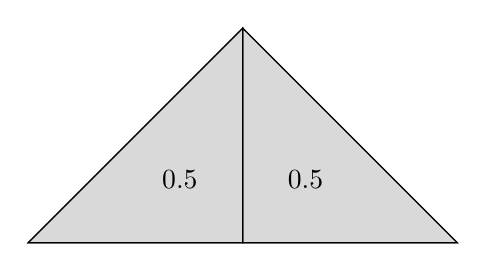
\begin{tikzpicture}[scale=2,baseline={([yshift={-\ht\strutbox}]current bounding box.north)},outer sep=0pt,inner sep=0pt]
                \gemsingem{0.5}{0}
            \end{tikzpicture}
            & The two gems are placed so that their tips touch the container's base and point toward each other. We assume $a_1 \ge \frac 1 2$ and normalize $a_1 + a_2$ to 1.\\

            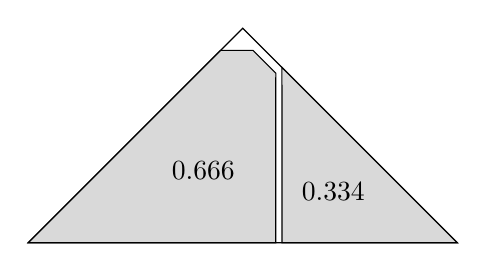
\begin{tikzpicture}[scale=2,baseline={([yshift={-\ht\strutbox}]current bounding box.north)},outer sep=0pt,inner sep=0pt]
                \gemsingem{0.334}{0}
            \end{tikzpicture}
            & They are then pushed as far to the left/right as possible. As $a_1$ grows, the gem becomes “cut-off” enough so that it does not overlap the container.\\

            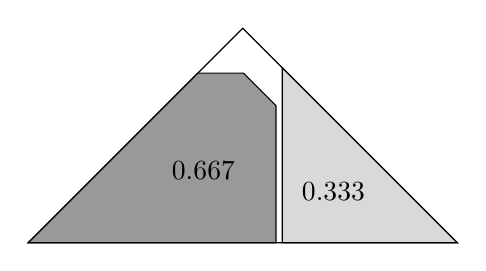
\begin{tikzpicture}[scale=2,baseline={([yshift={-\ht\strutbox}]current bounding box.north)},outer sep=0pt,inner sep=0pt]
                \gemsingem{0.333}{0}
            \end{tikzpicture}
            & As soon as $a_1 > \frac 2 3$, we know from \Cref{th:split-properties} that $b_1 = a_1$, so the gem takes the form of a sharp ruby from this point forward. We display it in a darker shade here.\\

            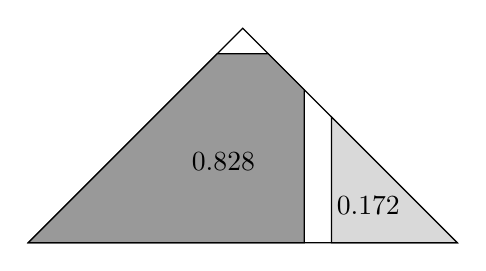
\begin{tikzpicture}[scale=2,baseline={([yshift={-\ht\strutbox}]current bounding box.north)},outer sep=0pt,inner sep=0pt]
                \gemsingem{0.172}{0}
            \end{tikzpicture}
            & When $a_1 = 2\s-2$, the ruby touches the container's right leg.\\

            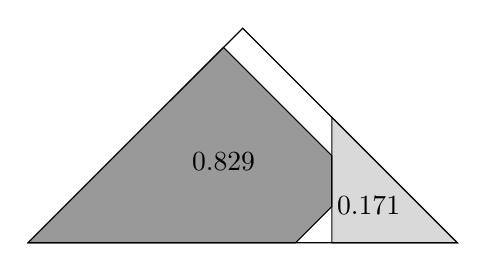
\begin{tikzpicture}[scale=2,baseline={([yshift={-\ht\strutbox}]current bounding box.north)},outer sep=0pt,inner sep=0pt]
                \gemsingem{0.171}{0}
            \end{tikzpicture}
            & So when the ruby gets larger than that, it has to be rotated so that its tip points up. That these two positions exactly fit is the defining property of the ruby shape.\\

            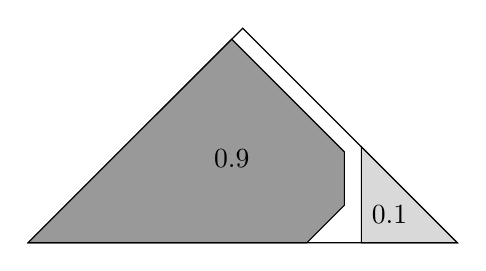
\begin{tikzpicture}[scale=2,baseline={([yshift={-\ht\strutbox}]current bounding box.north)},outer sep=0pt,inner sep=0pt]
                \gemsingem{0.1}{0}
            \end{tikzpicture}
            & In this orientation, it can then grow without overlapping the container and the smaller gem.\\

            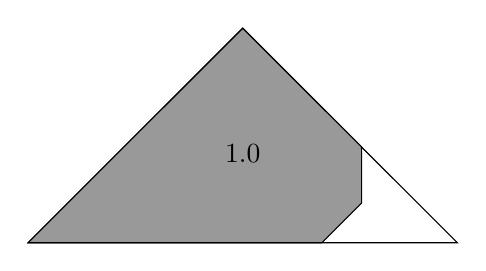
\begin{tikzpicture}[scale=2,baseline={([yshift={-\ht\strutbox}]current bounding box.north)},outer sep=0pt,inner sep=0pt]
                \gemsingem{0}{0}
            \end{tikzpicture}
            & When $a_1 = 1$, the ruby touches all sides of the container triangle.\\
        \end{tabular}
    \end{table}

    The smaller gem is always placed so that its tip touches the bottom of the container gem and its left corner fits into the containers right corner. By assumption, its incircle is smaller than $\nicefrac{1}{2}$, so it will fit inside the right half of the container and thus never overlap the container's boundary. For the larger gem, there are three cases:

    \paragraph{Case 1}

    When $a_1 \le \frac{2}{3}$, we know from \Cref{th:split-properties} that $b_1 \ge 2a_1 - 1$. We have to show that the corner-width of our gem does not exceed the diagonal of the container:

    \begin{align*}
        W(a_1, 2a_1-1) &\le D(1)\\
        \\
        \iff (2+2\s)\sqrt{\frac{a_1}{\pi}} - \frac{(2+\s)(2\sqrt{\s-1}-1)}{\sqrt{2(\s-1)\pi}}\sqrt{2a_1-1} &\le \frac{2+\s}{\sqrt{\pi}}
    \end{align*}

    Expressions of the form $f\sqrt{x} - g\sqrt{2x-1}$ have their only extremum at $x = \frac{f^2}{2(f^2-2g^2)}$. This point turns out to be a global minimum for $f,g > 0$.
    In our case, this minimum point is at $a_1 = \frac{1+5\s+4\sqrt{1+5\s}}{35} \approx 0.5553$.
    As we can check our inequality to be true for $a_1 = \frac{1}{2}$ as well as for $a_1 = \frac 2 3$, this means that it always holds between those two values.

    \paragraph{Case 2}

    In the range $\frac{2}{3} \le a_1 \le 2\s-2$, we know from \Cref{th:split-properties} that $b_1 = a_1$, essentially making the gem into sharp a ruby. We have to show that the corner-width of the ruby is always smaller than the diagonal of the container:

    $$W(a_1, a_1) \le D(1)$$

    But in the range for $a_1$ specified above, this is true:

    $$W(a_1, a_1) = \frac{(1+\s)^{\frac{3}{2}}}{\sqrt{\pi}}\sqrt{a_1} \le \frac{(1+\s)^{\frac{3}{2}}}{\sqrt{\pi}}\sqrt{2\s-2} = \frac{2+\s}{\sqrt{\pi}} = D(1)$$

    In both Case 1 and Case 2, the two gems do not overlap each other because the projections of their incircles do not overlap. See \Cref{th:hats-in-iso} for a proof.

    \paragraph{Case 3}

    For $a_1 = 2\s-2$, the ruby touches the containers right leg.
    When $2\s-2 < a_1 \le 1$, it is no longer possible to place the gem like before without overlapping the container. In this case, we rotate it so that its bottom touches the bottom of the container gem and push it as far left as possible.

    This is actually the defining property for the shape of the ruby: The cut-off is exactly so large that, when the growing ruby touches the container, the remaining space left over by the smaller gem is a (symmetric) kite, so that the ruby can be rotated.

    In this orientation, it will never overlap the container: It can be enclosed in a (non-cut) $(a_1, 0)$-gem, with the same rotation as the container gem, and $a_1 \le 1$, so our ruby always fits inside the container gem.

    To show that the ruby does not overlap the smaller gem, we have to show that the following inequality holds for $2\s-2 \le a_1 \le 1$: The corner-width of the ruby, added to the diagonal of the small gem, must not exceed the container's width:

    \begin{align*}
        W(a_1,a_1) + D(1-a_1) &\le w(1,0)\\
        \\
        \iff (2+2\s)\sqrt{\frac{a_1}{\pi}} - \frac{(2+\s)(2\sqrt{\s-1}-1)}{\sqrt{2(\s-1)\pi}}\sqrt{a_1} + \frac{2+\s}{\sqrt{\pi}}\sqrt{1-a_1} &\le \frac{2\s + 2}{\sqrt{\pi}}\\
        \\
        \iff \frac{(1+\s)^{\frac{3}{2}}}{\sqrt{\pi}}\sqrt{a_1} + \frac{2+\s}{\sqrt{\pi}}\sqrt{1-a_1} &\le \frac{2\s + 2}{\sqrt{\pi}}
    \end{align*}

    Expressions of the form $f\sqrt{x} + g\sqrt{1-x}$ have their only extremum at $x = \frac{f^2}{f^2+g^2}$. This point turns out to be a global maximum for $f,g > 0$. In our case, the maximum is at $\frac{1+2\s}{7} \approx 0.5469$, and we have equality for $a_1 = 2\s-2 \approx 0.8284$. If $a_1$ gets larger than that, the left hand side of the equation will only get smaller, so that the inequality holds. This concludes the proof of \Cref{th:gems-in-gem}.
\end{proof}

Like with hats, “rounding” the container gem to a sharp gem with larger cut-off does not affect the packing properties:

\begin{lemma}\label{th:rounded-gems-in-gem}
    Any two $(a, b, (1,1))$-conjugated sharp gems can be packed into a sharp $(a,b)$-gem.
\end{lemma}

\begin{proof}
    \Cref{th:gems-in-gem} tells us that this theorem is true for $b = 0$. 
    For $b > 0$, we flip the containers cut-off corner to the right, and also flip the smaller gem's cut-off corner so that it points to the right. Because the cut-off has the same shape, the inner gems will not overlap the container.
\end{proof}

\fig{gems-rounding}{Cutting one corner of each gem by the same value does not affect the packing.}

\begin{theorem}\label{th:sharp-gem}
    Any sharp ruby instance $S \in \S(a,b)$ can be packed into a sharp $(a,b)$-gem.
\end{theorem}

\begin{proof}
    By \Cref{th:hats-in-iso} and the Split Packing Theorem.
\end{proof}

As a minor corollary, since rubies are subsets of sharp rubies of the same incircle, we can state the same property for regular rubies.

\begin{theorem}\label{th:gem}
    Any ruby instance $R \in \R(a,b)$ can be packed into an $(a,b)$-gem.
\end{theorem}

\begin{proof}
    This follows analogously to the reasoning with sharp gems. In this case, when cutting off the corners of the container gem, all corners of the contained gems are cut off by the same value, so they still fit inside.
\end{proof}

\section{Isosceles right triangles}

As isosceles right triangles are simply non-rounded sharp gems, this is again going to be a short section.

\begin{theorem}\label{th:iso-right}
    Given an isosceles right triangle with an incircle of area $a$, all sharp ruby instances with a combined incircle area of up to $a$ can be packed into the triangle, and this area bound is tight.
    See \Cref{fig:example-sharp-rubies-in-iso} for some example packings.
    Expressed algebraically, the critical density is

    $$4\sqrt{2(\s-1)} + 3\s -7 \approx 88.34\%.$$

\end{theorem}

\begin{proof}
    The triangle is a sharp $(a,0)$-gem, and by \Cref{th:gem} we can pack any sharp ruby instance $S \in \myS(a)$ into such a gem.

    A sharp ruby with an incircle area of more than $a$ cannot be packed, as its incircle would be larger than the triangle's incircle.

    The critical density can be calculated using the area of sharp rubies mentioned above.
\end{proof}

\begin{figure}
    \begin{tabular}{cc}
        \subfig[0.0085]{example-sharp-rubies-in-iso-1} &
        \subfig[0.0085]{example-sharp-rubies-in-iso-2} \\
        \subfig[0.0085]{example-sharp-rubies-in-iso-3} &
        \subfig[0.0085]{example-sharp-rubies-in-iso-4} \\
        \subfig[0.0085]{example-sharp-rubies-in-iso-5} &
        \subfig[0.0085]{example-sharp-rubies-in-iso-6} \\
    \end{tabular}
    \caption{Example packings of various sharp ruby instances in an isosceles right triangle produced by Split Packing.}
    \label{fig:example-sharp-rubies-in-iso}
\end{figure}

We can make the following observation here: Given an isosceles right triangle with an incircle area of $a$, and some arbitrary objects, if one can enclose each object in a sharp ruby, and the combined incircle area of these rubies is not larger than $a$, then the objects can be packed into the triangle. This is a very general result which can be used to directly solve some other interesting packing problems:

\begin{corollary}\label{th:iso-right2}
    Given a right isosceles triangle with an incircle area of $a$, the following object instances can be packed into the square.

    \begin{itemize}
        \item All circle instances with a combined area of up to $a$,
        \item all octagon instances with a combined area of up to $\frac{8\s-8}{\pi}a \approx 1.0548a$, and
        \item all square instances with a combined area of up to $\frac{3+2\s}{2\pi}a \approx 0.9276a$, which is also exactly half of the square's area.
    \end{itemize}

    All of these area bounds are tight. See \Cref{fig:example-stuff-in-iso} for some example packings.
\end{corollary}

\begin{proof}
    As demonstrated above, the three shapes are subsets of rubies in these specific area ratios. To pack them, enclose all of them in the smallest possible sharp ruby. The combined incircle area of these rubies will now be at most $a$. We then know from \Cref{th:iso} that we can always pack these rubies.

    The tightness of these bounds is obvious for circles and hexagons. For squares, the tightness follows from the result by \textcite{gobel1979geometrical} that the largest two squares that can be packed (with rotation) into a square are quarter-squares. This implies that, when cutting the square along its diagonal, there is no larger square that can be packed into an isosceles right triangle than one with half the triangle's area.
\end{proof}

\begin{figure}
    \begin{tabular}{cc}
        \subfig[0.0085]{example-stuff-in-iso-1} &
        \subfig[0.0085]{example-stuff-in-iso-2} \\
        \subfig[0.0085]{example-stuff-in-iso-3} &
        \subfig[0.0085]{example-stuff-in-iso-4} \\
    \end{tabular}
    \caption{Example packings of ruby-, circle-, octagon-, and square instances in an isosceles right triangle produced by Split Packing.}
    \label{fig:example-stuff-in-iso}
\end{figure}

\section{Squares}

Finally, we turn to square containers. Having established $(a,b)$-gems as $\R(a,b)$-shapes, to argue about the packing properties of squares is going to be relatively straightforward. We first argue about the worst-case instance for squares:

\begin{lemma}\label{th:square-worst}
    Two touching equal circles, packed into opposing corners of a square, are the squares \emph{twincircles}, meaning that there are no two larger equal circles which can be packed.
\end{lemma}

\begin{proof}
    This can be proven similarly like in \Cref{th:iso-worst}: Let $r$ be the radius of these circles. When eroding the square by $r$, the result is a square with a diagonal of $2r$. When eroding by a larger radius $r + \varepsilon$, the diagonal will be smaller than $2r$. But the centers of the two circles need to be placed at least $2r + 2\varepsilon$ away from each other, and additionally need a distance of at least $r + \varepsilon$ from the square's boundary. We see that both constraints cannot be satisfied at the same time.
\end{proof}

\begin{lemma}\label{th:square-twincircle-area}
    The twincircles of a square with area $a$
    have a combined area of
    $$\frac{\pi}{3+2\s}a \approx 0.5390a.$$
\end{lemma}

\begin{proof}
    We can construct the twincircles' radius $r$ as seen in \Cref{fig:square-worst-construction}:

    \begin{equation*}
        2r + 2\frac{r}{\s} = \sqrt{a} \iff r = \frac{\sqrt{a}}{2 + \s}
    \end{equation*}

    So, the combined area of the twincircles is

    $$2\pi r^2 = 2\pi\frac{a}{4 + 4\s + 2} = \frac{\pi}{3+2\s}a.$$
\end{proof}

\fig[5]{square-worst-construction}{Constructing the twincircles' radius $r$.}

Note that in the next lemma, we no longer pack \emph{sharp} gems, but regular gems, whose two corners are cut off. The reason it will become clear in \Cref{fig:gems-in-square}: A large sharp $(a,0)$-ruby cannot be packed into the square.

\begin{lemma}\label{th:gems-in-square}
    Any two $(a,0,(1,1))$-conjugated gems can be packed into a square with twincircle area $a$.
\end{lemma}

\begin{figure}
    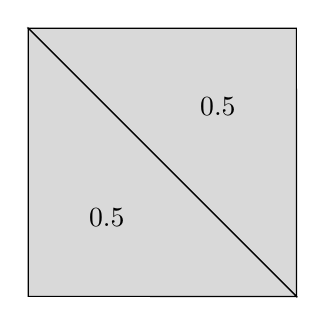
\begin{tikzpicture}[scale=2.5]
        \gemsinsquare{0.5}
    \end{tikzpicture}
    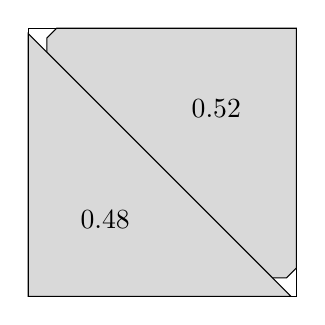
\begin{tikzpicture}[scale=2.5]
        \gemsinsquare{0.48}
    \end{tikzpicture}
    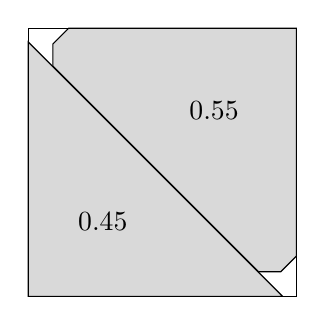
\begin{tikzpicture}[scale=2.5]
        \gemsinsquare{0.45}
    \end{tikzpicture}
    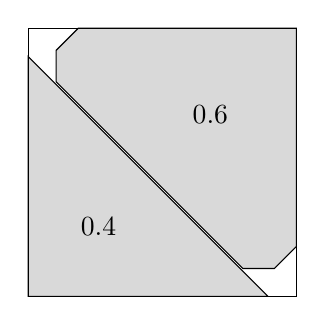
\begin{tikzpicture}[scale=2.5]
        \gemsinsquare{0.4}
    \end{tikzpicture}

    \vspace{5mm}

    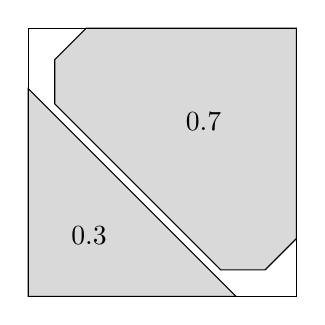
\begin{tikzpicture}[scale=2.5]
        \gemsinsquare{0.3}
    \end{tikzpicture}
    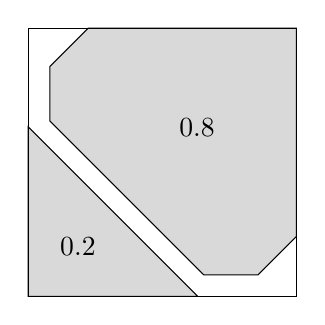
\begin{tikzpicture}[scale=2.5]
        \gemsinsquare{0.2}
    \end{tikzpicture}
    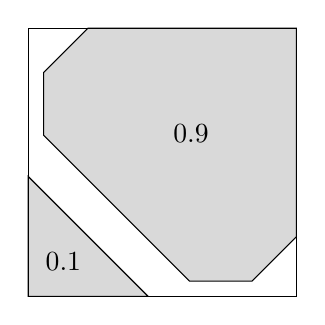
\begin{tikzpicture}[scale=2.5]
        \gemsinsquare{0.1}
    \end{tikzpicture}
    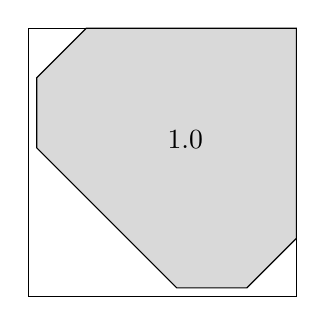
\begin{tikzpicture}[scale=2.5]
        \gemsinsquare{0}
    \end{tikzpicture}

    \caption{Hat-in-square packings for different values of $a_1$ and $a_2$}
    \label{fig:gems-in-square}
\end{figure}

\begin{proof}
    Place the tips of the gems in two opposing corners of the square, like in \Cref{fig:gems-in-square}.
    This placement constitutes a valid packing because (1) the gems fit into the square individually and (2) the gems never overlap. This can be proven algebraically in exactly the same fashion as in \Cref{th:gems-in-gem}, where we proved a similar statement about packing into gems.
\end{proof}

\begin{theorem}\label{th:square}
    Given a square with a twincircle area of $a$, all ruby instances with a combined incircle area of up to $a$ can be packed into the square, and this area bound is tight.
    See \Cref{fig:example-rubies-in-square} for some example packings.
    Expressed algebraically, the critical density for the rubies' ares is

    $$8\sqrt{2(\s-1)}+6\s-15 \approx 76.67\%.$$
\end{theorem}

\begin{proof}
    By \Cref{th:gems-in-square} and the Split Packing Theorem, the square is a $\R(a)$-shape.

    Two rubies with a combined incircle area of more than $a$ will have incircles which are larger than the square's twincircles. As shown in \Cref{th:square-worst}, those cannot be packed, which means that the rubies cannot be packed, as well.

    The critical density can be calculated using the area of the rubies' incircles (see \Cref{th:square-twincircle-area}).
\end{proof}

\begin{figure}
    \begin{tabular}{cc}
        \subfig[0.017]{example-rubies-in-square-1} &
        \subfig[0.017]{example-rubies-in-square-2} \\
        \subfig[0.017]{example-rubies-in-square-3} &
        \subfig[0.017]{example-rubies-in-square-4} \\
        \subfig[0.017]{example-rubies-in-square-5} &
        \subfig[0.017]{example-rubies-in-square-6} \\
    \end{tabular}
    \caption{Example packings of various ruby instances in a square produced by Split Packing.}
    \label{fig:example-rubies-in-square}
\end{figure}

At this point, we can make a similar observation like for isosceles right triangles: Given a square with a twincircle area of $a$, and some arbitrary objects, if one can enclose each object in a ruby, and the combined incircle area of these rubies is not larger than $a$, then the objects can be packed into the square. This is a very general result which can be used to directly solve some other interesting packing problems:

\begin{corollary}\label{th:square2}
    Given a square with a twincircle area of $a$, the following object instances can be packed into the square.

    \begin{itemize}
        \item All circle instances with a combined area of up to $a$,
        \item all octagon instances with a combined area of up to $\frac{8\s-8}{\pi}a \approx 1.0548a$, and
        \item all square instances with a combined area of up to $\frac{3+2\s}{2\pi}a \approx 0.9276a$, which is also exactly half of the square's area.
    \end{itemize}

    All of these area bounds are tight. See \Cref{fig:example-stuff-in-square} for some example packings.
\end{corollary}

\begin{proof}
    As demonstrated above, the three shapes are subsets of rubies in these specific area ratios. To pack them, enclose all of them in the smallest possible ruby. The combined incircle area of these rubies will now be at most $a$. We then know from \Cref{th:square} that we can always pack these rubies.

    The tightness of these bounds for circles was shown in \Cref{th:square-twincircle-area}. For the same reason, two octagons with larger incircles cannot be packed: Their incircles would overlap, which means that the octagons themselves would overlap. For squares, the fact that the largest two squares that can be packed into a square (with rotation) are two quarter-squares was shown by \textcite{gobel1979geometrical}.
\end{proof}

\begin{figure}
    \begin{tabular}{cc}
        \subfig[0.017]{example-stuff-in-square-1} &
        \subfig[0.017]{example-stuff-in-square-2} \\
        \subfig[0.017]{example-stuff-in-square-3} &
        \subfig[0.017]{example-stuff-in-square-4} \\
    \end{tabular}
    \caption{Example packings of ruby-, circle-, octagon-, and square instances in a square produced by Split Packing.}
    \label{fig:example-stuff-in-square}
\end{figure}

Note that the result that you can pack all sets of squares with a density of up to $\nicefrac 1 2$ is already known, even without rotations, as it can be done with Moon \& Moser's Shelf Packing approach \cite{MM1967some}. For circles and octagons, to our knowledge, this is a new result.

\chapter{Future work}\label{ch:future-work}

We see many opportunities to apply the techniques behind Split Packing in the context of other packing and covering problems.

In this thesis, we mainly considered triangular and square containers. It would be interesting to see whether the Split Packing approach could be adapted to even \textbf{more container types}, like circles, ovals, regular polygons, or generalized quadrilaterals. For some of these container types, even the worst-case instance does not seem obvious. For circular and “almost square” rectangular containers, we assume the worst cases would again be their twincircles, see \Cref{fig:circle-rect-worst}, but it is unclear how to deal with the resulting shapes when cutting along the circles' tangent: Compared to triangular and square containers, these shapes cannot be split into self-similar pieces. It is also possible that the depicted instances are not the actual worst cases.

\fig[1.5]{circle-rect-worst}{Assumed worst-case instances for a circle and a near-square rectangle.}

Also, the problem of finding the critical density for packing into \textbf{acute triangles} is still open. See \Cref{sec:acute-triangles} for a discussion on why the Split Packing approach does not directly work for acute ones. A strategy for packing acute triangles with critical density, combined with the results of this thesis, would give an elegant, general result for all triangles.

Instead of packing circular, square, and octagonal objects, \textbf{more object types} could be considered, like ovals, rectangles, or even more general convex objects. For these modified problems, again, it does not seem obvious what the worst-case packings would look like.

For long rectangles (and long containers in general), in \Cref{sec:rectangles} we discussed that the maximally packable area is limited by the relatively small height, making the problem rather trivial. It would be a more interesting problem to require a \textbf{maximum object size}: What is the largest $a$ so that all circle instances with a combined area of at most $a$, each of which have a diameter \emph{not larger than a rectangle's smaller side}, can be packed into that rectangle?

The Split Packing method as described in this thesis is a strictly offline approach, as the greedy splitting requires sorting the complete input instance, and then proceeds in a top-down fashion. It would be interesting to study to which extent the obtained results could be replicated in an \textbf{online situation}. The best algorithm that packs squares into a square in an online fashion is currently by \textcite{brubach2014improved} and gives a density guarantee of $\frac{2}{5}$. As mentioned in \Cref{sec:related-squares}, we can directly use this algorithm to pack circles into a square in an online situation with a density of $\frac{\pi}{10} \approx 0.3142$. It would be particularly interesting to see whether some form of online Split Packing would give better results.

Our original motivation stemmed from origami design. When only packing circles, the resulting origami structures resemble arbitrary stars. When one wants to design general tree-shaped structures, it is necessary to introduce separating pathways between the circles, a technique called \textbf{circle/river packing}, pioneered by \textcite{lang1996computational}.
A packing scheme like Split Packing seems promising because it often introduces gaps inbetween two subgroups anyway. At this point, we can establish a constant-factor approximation for perfectly symmetric binary trees (see \Cref{fig:origami}), but we do not know how to approximate the paper size needed for crease patterns of general trees.

\fig[8]{origami}{A folding of the tree on the left can be realized by a crease pattern based on the circle/river packing on the right.}

It seems like a natural extension to apply Split Packing to \textbf{three-dimensional packing} problems. For example, one could try to pack spheres into a cube using a Split Packing approach. Unfortunately, this does not directly seem to work out: Assuming the worst case are two equally sized spheres packed into opposite corners of the cube, one would like to be able to cut the cube along the spheres' tangential plane. This results in two shapes like depicted on the right in \Cref{fig:cube-half}, but it is not possible to fit two quarter-spheres into each of these polyhedra. Still, any extensions regarding three dimensional problems would be notable.

\begin{figure}
    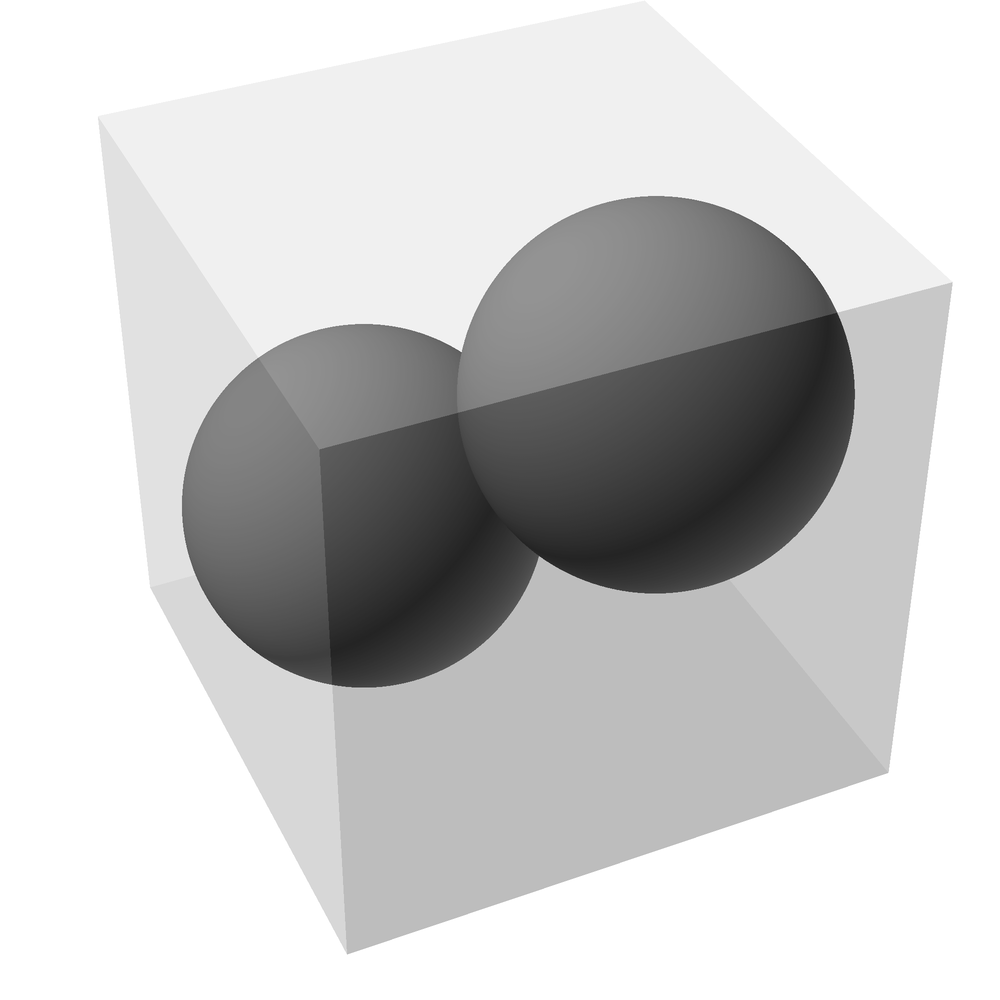
\includegraphics[width=0.45\textwidth]{cube.png}
    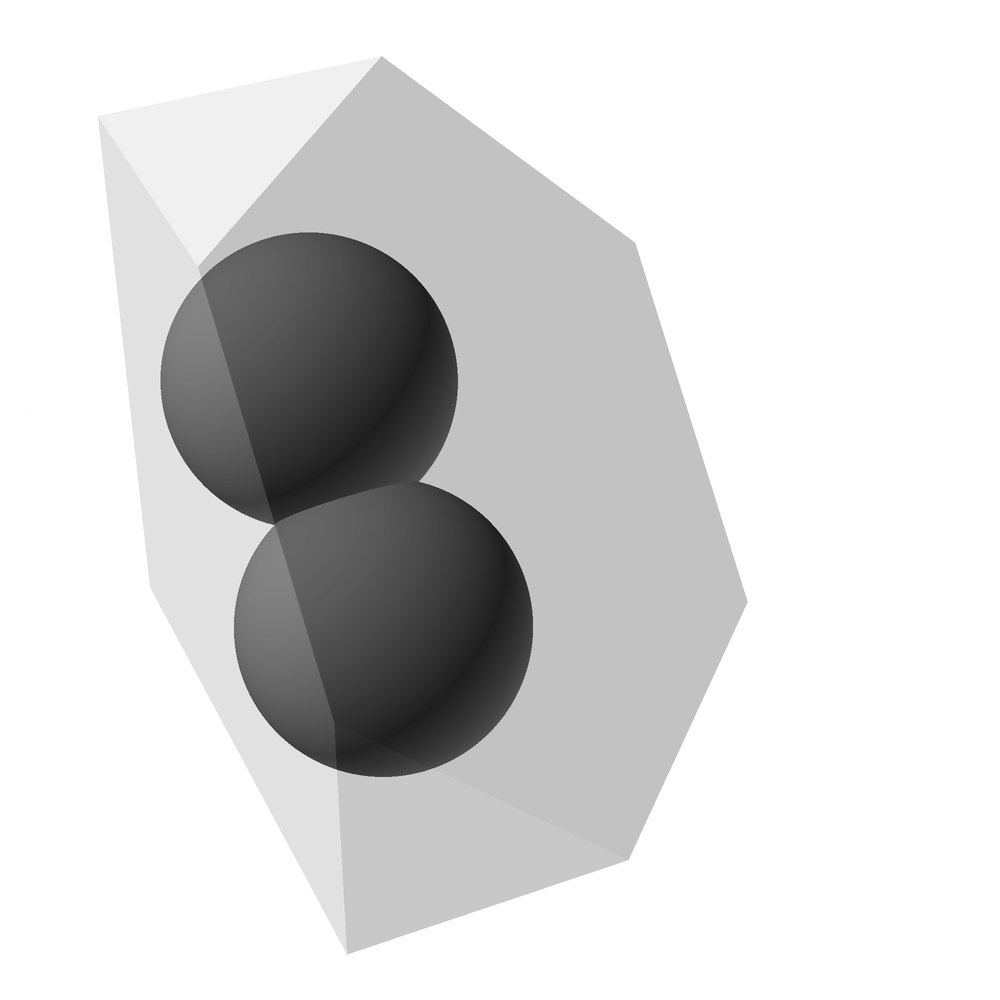
\includegraphics[width=0.45\textwidth]{cube-half.png}
    \caption{Left: Assumed worst case for packing spheres into a cube. Right: Two quarter-spheres do not fit in a half.}\label{fig:cube-half}
\end{figure}

Instead of packing circles into containers, one could ask a question which is in some sense the opposite problem: What is the smallest area so that we can always \textbf{cover the container} with circles of that combined area? For example, if we want to cover an isosceles right triangle, and restrict ourselves to at most two circles in our input instance, the area of a circle whose diameter equals the triangle's hypotenuse is sufficient, see \Cref{fig:cover}. It would now be necessary to show that the area of the left circle is always enough to cover the quadrilateral on the left, and it does not seem trivial to find an argument fot that.

\fig[1.5]{cover}{An isosceles right triangle can always be covered by two circles with a combined area of its excircle.}

\printbibliography

\end{document}
